% Exemplo de relat?rio t?cnico do IC
% Criado por P.J.de Rezende antes do Alvorecer da Hist?ria.
% Modificado em 97-06-15 e 01-02-26 por J.Stolfi.
% Last edited on 2003-06-07 21:12:18 by stolfi

% modificado em 1o. de outubro de 2008

\documentclass[11pt,twoside]{article}
%\usepackage{techrep-ic}
\usepackage[sort&compress]{natbib}
\usepackage[english]{babel}
\usepackage{largepages}
\usepackage{amssymb}
\usepackage{graphicx,url}
\usepackage{makeidx}
\usepackage{listings}
%% SE USAR CODIFICA??O LATIN1, TROQUE AS ATIVA??ES DOS DOIS COMANDOS A
%% SEGUIR:
\usepackage[latin1]{inputenc}
\usepackage{rotating}
%\usepackage[utf-8]{inputenc}

\makeindex

\begin{document}

%%% P?GINA DE CAPA %%%%%%%%%%%%%%%%%%%%%%%%%%%%%%%%%%%%%%%%%%%%%%%
% 
% N?mero do relat?rio
%\TRNumber{45}

% DATA DE PUBLICA??O (PARA A CAPA)
%
%\TRYear{11}  % Dois d?gitos apenas
%\TRMonth{5} % Num?rico, 01-12

% LISTA DE AUTORES PARA CAPA (sem afilia??es).
%\TRAuthor{L.P. Tizzei \and C.M.F. Rubira}

% T?TULO PARA A CAPA (use \\ para for?ar quebras de linha).
%\TRTitle{Public Health Complaint Software Product Line}

%\TRMakeCover

%%%%%%%%%%%%%%%%%%%%%%%%%%%%%%%%%%%%%%%%%%%%%%%%%%%%%%%%%%%%%%%%%%%%%%
% O que segue ? apenas uma sugest?o - sinta-se ? vontade para
% usar seu formato predileto, desde que as margens tenham pelo
% menos 25mm nos quatro lados, e o tamanho do fonte seja pelo menos
% 11pt. Certifique-se tamb?m de que o t?tulo e lista de autores
% est?o reproduzidos na ?ntegra na p?gina 1, a primeira depois da
% p?gina de capa.
%%%%%%%%%%%%%%%%%%%%%%%%%%%%%%%%%%%%%%%%%%%%%%%%%%%%%%%%%%%%%%%%%%%%%%

%%%%%%%%%%%%%%%%%%%%%%%%%%%%%%%%%%%%%%%%%%%%%%%%%%%%%%%%%%%%%%%%%%%%%%
% Nomes de autores ABREVIADOS e titulo ABREVIADO,
% para cabe?alhos em cada p?gina.
%
\markboth{}{Public Health Complaint Software Product Line}
\pagestyle{myheadings}

%%%%%%%%%%%%%%%%%%%%%%%%%%%%%%%%%%%%%%%%%%%%%%%%%%%%%%%%%%%%%%%%%%%%%%
% T?TULO e NOMES DOS AUTORES, completos, para a p?gina 1.
% Use "\\" para quebrar linhas, "\and" para separar autores.
%
\title{Public Health Complaint Software Product Line}

\author{
Leonardo Pondian Tizzei\thanks{Institute of Computing - University of Campinas - e-mail: \texttt{tizzei@ic.unicamp.br}} \and
%Bruno Iizuka\thanks{Institute of Computing - University of Campinas} \and
%Renato Manzoni\thanks{Institute of Computing - University of Campinas} \and
%Amanda Nascimento\thanks{Institute of Computing - University of Campinas} \and
Cec\'{i}lia Mary Fischer Rubira\thanks{Institute of Computing - University of Campinas - e-mail: \texttt{cmrubira@ic.unicamp.br}}
}

\date{\today}

\maketitle
%%%%%%%%%%%%%%%%%%%%%%%%%%%%%%%%%%%%%%%%%%%%%%%%%%%%%%%%%%%%%%%%%%%%%%
\newpage
\tableofcontents

%%%%%%%%%%%%%%%%%%%%%%%%%%%%%%%%%%%%%%%%%%%%%%%%%%%%%%%%%%%%%%%%%%%%%%
\newpage

\begin{abstract} 
  
\end{abstract}



\section{Introduction}

%context
\textit{Software product line} (SPL) engineering is a paradigm to develop software applications using core assets and mass
customization~\cite{Pohl:2005:SPL}. The extractive
adoption of a SPL capitalizes on existing system~\cite{Lee:2009:ERU}, and focuses on reusing software assets of existing products in order to reduce
costs. This approach is very
appropriate when the collection of products has a significant amount of commonality and differences among them~\cite{Krueger:2002:ETS}. The
Feature-oriented reengineering process
is an example of extractive approach, which provides guidelines to build a SPL from legacy software assets by using feature model to support the
creation of other development
assets, such as the product line architecture~\cite{Kang:2006:FOR}. Feature model is usually applied to represent the commonalities and variabilities
of a SPL. 

Aspect-oriented Programming (AOP) can support extractive SPL adoption by inserting variability on existing components and by wrapping crosscutting
concerns~\cite{Truyen:2000:ART}.
Crosscutting concerns are concerns that cut across other concerns and are responsible for producing tangled representations that are difficult to
understand and
maintain~\cite{Rashid:2003:MCA}. AOP can facilitate the integration of existing components by implementing glue-code~\cite{Kvale:2005:CSB}.
Furthermore, there are evidences that the use of aspects supports the design of stable PLA~\cite{Figueiredo:2008:ESP,
Tizzei:2011:ECSA,Tizzei:2011:CMA}. However, existing
feature-oriented reengineering approaches does not provide support for aspect-oriented techniques.

We propose a feature-oriented product line approach, which uses aspect-oriented techniques to support separation of concerns throughout the adoption
process. Instead of creating
the entire approach from scratch, as feature-oriented software development is a solid discipline we combined existing feature-oriented approaches to
achieve our goal. When
necessary, we also extended feature-oriented techniques to support reasoning about crosscutting concerns. 

As integrating existing techniques is a difficult task, we performed an exploratory case study to assess the feasibility of our approach. Three legacy
applications from the
same domain have been chosen and we have executed the approach to produce a software product line from which three products can be derived, one for
each corresponding legacy
application. Another objective of the case study is to promote empirical studies with product lines, since there is lack of empirical studies in this
area. Award-winning product
lines are usually commercial systems which are not publicly available for conducting research~\cite{Couto:2011:SMR}. Therefore, we made available all
artifacts (e.g. feature
diagrams, architecture, source codes) produced for the product line adoption.

\section{Reverse engineering}
The reverse engineering phase is important to capitalize on existing artifacts~\cite{Lee:2009:ERU}. Models such as architectures and
component specification support developers and domain analysts to understand legacy applications and understanding is a key factor
for reuse~\cite{Frakes:1996:SRM}. Figure~\ref{fig:reverseEngineering} shows the main activities of reverse engineering phase, which is based
on Lee et al.~\cite{Lee:2009:ERU}. 

\begin{figure}[!htb]
   \centering
   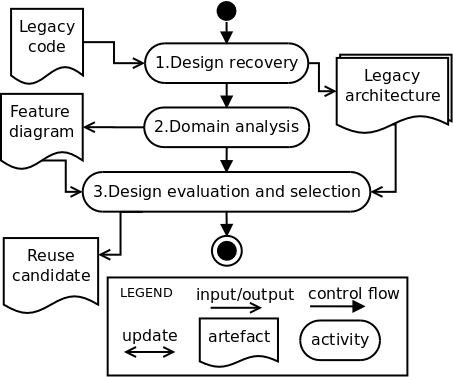
\includegraphics[scale=0.4]{figs/reverseEngineering-v01.png}
   \caption{Reverse engineering activities}
   \label{fig:reverseEngineering}
\end{figure}

\subsection{Design Recovery}
\label{sec:designRecovery}
The \textit{Design recovery} activity can be supported by CASE tools such as Enterprise
Architect~\footnote{http://www.sparxsystems.com/products/ea/downloads.html}. The result of this activity is a set of legacy architectures
for each corresponding application.

\begin{figure}[h!t!b!]
   \centering
    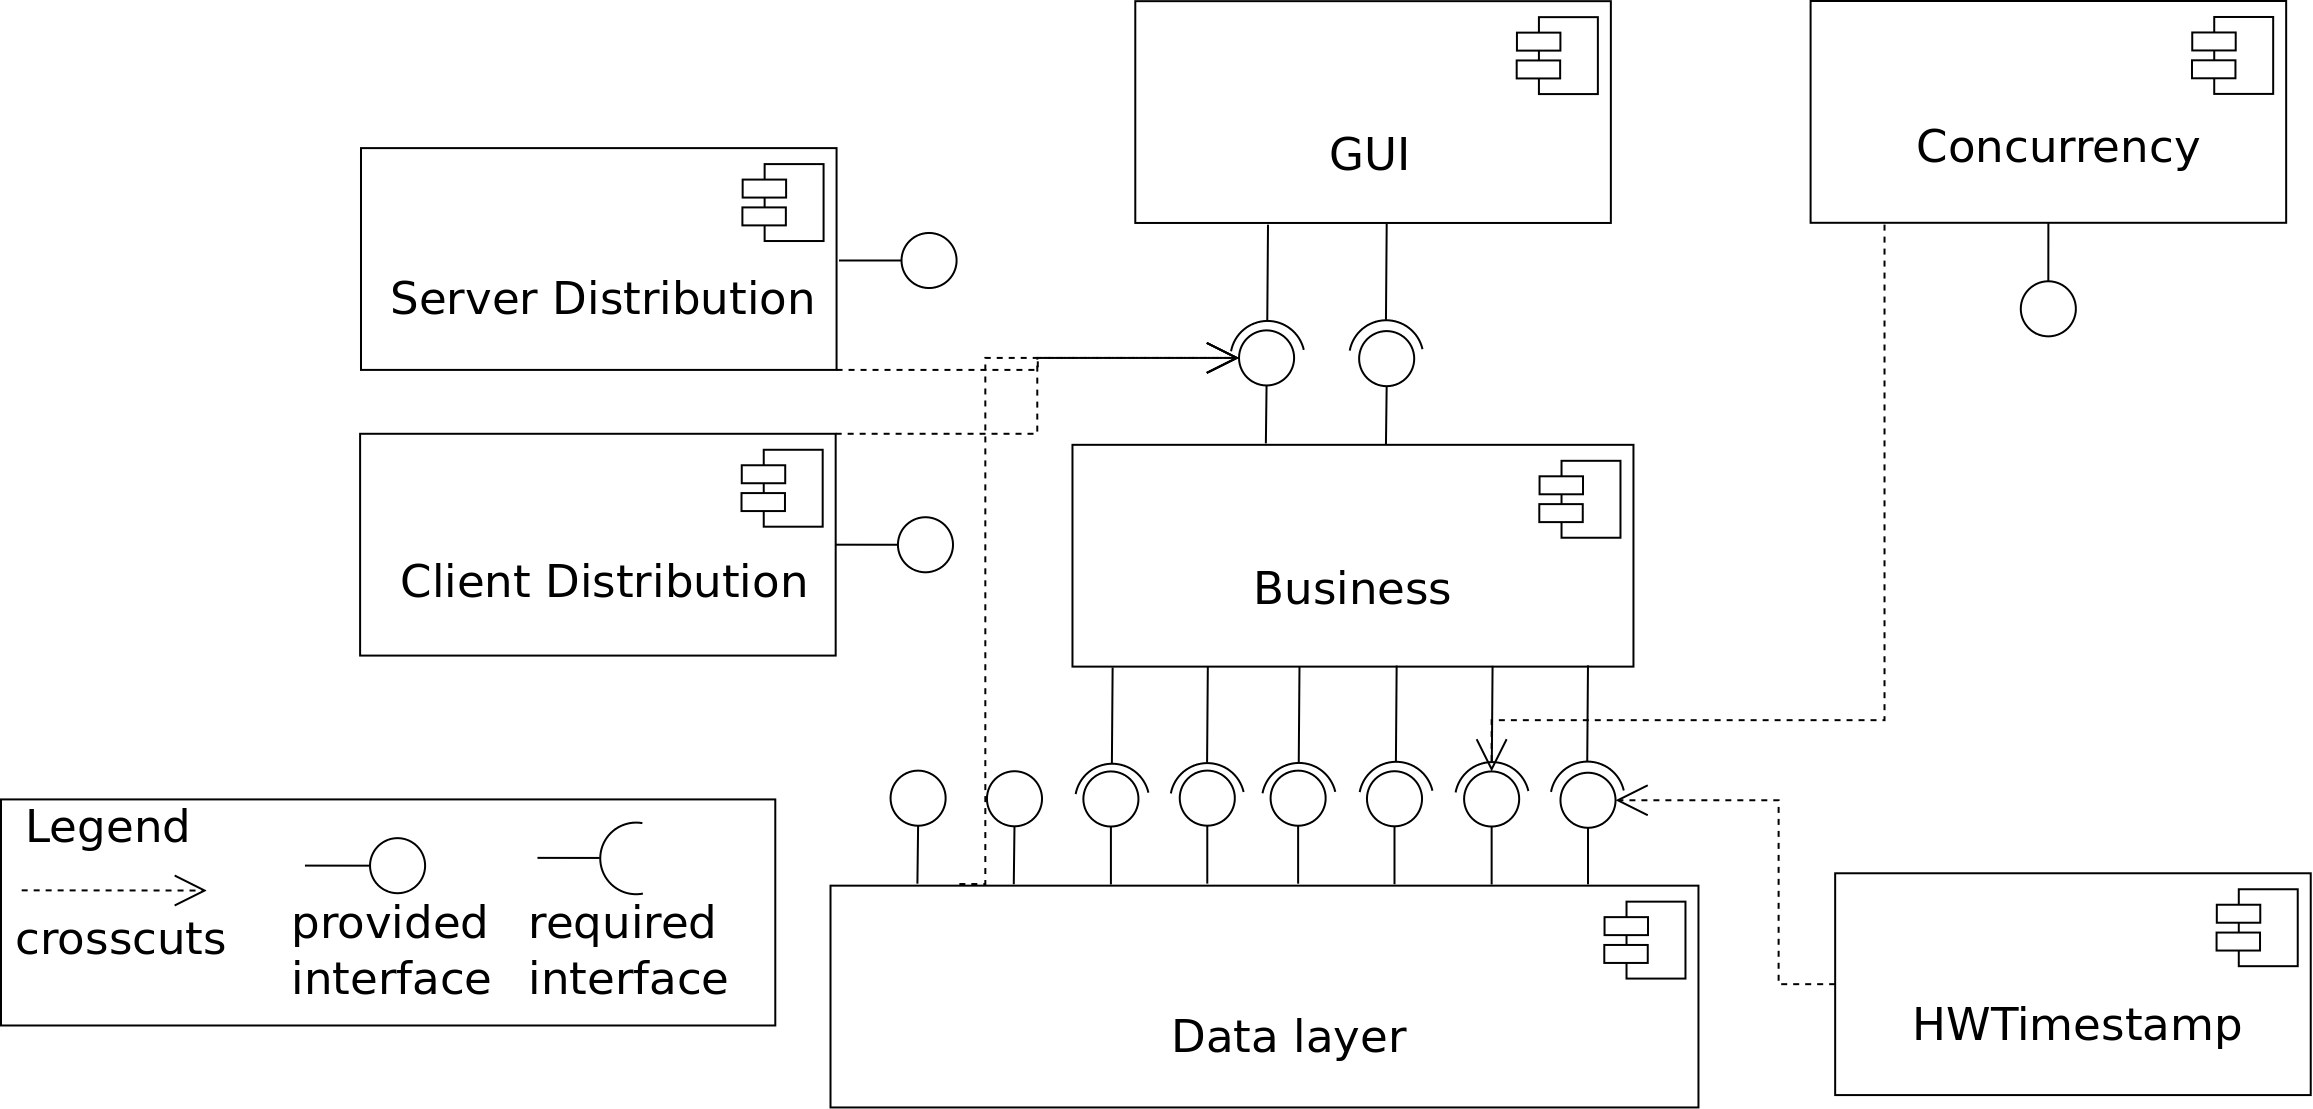
\includegraphics[scale=0.13]{figs/legacyHW-architecture.png}
   \caption{Component-based Architecture of Legacy Healthwatcher (based on Healthwatcher legacy architecture~\cite{hw-arch})}
   \label{fig:recoveredArch}
\end{figure}


\subsection{Domain Analysis}
\label{sec:domainAnalysis}
\textit{Domain analysis} defines product line features based on legacy application features and market needs~\cite{Kang:2006:FOR}, that is,
legacy application features can be removed or changed and new features can be added due to market needs. Thus,
both features that have been implemented and features that will be implemented must be represented in the feature diagram. In order to
create the feature diagram, it is important to define an initial set of intended products for product line as well as their intended
commonalities and variabilities~\cite{Pohl:2005:SPL}. The feature diagram has been created according to the guidelines proposed by Lee
et al.~\cite{Lee:2002:CGF}. Previous models and documents (e.g. requirements, use cases specification), and
existing artifacts (e.g. users manual, the application itself) can also be useful to identify features~\cite{John:2003:ERU}.             
Figure~\ref{fig:featureDiag} shows the feature diagram of the Public Health Complaint SPL. We identified the features based on use case
specification (e.g. Healthwatcher use cases~\cite{hw-usecase})  and on the use of the legacy applications (i.e. Healthwatcher,
Medwatch~\cite{medwatch}, and DPH-LA~\cite{dphla}). Feature variability should be consistent with use case variability. The relationship
among features is further specified in Section~\ref{sec:featGroups}.



\begin{figure}[!h!t!b]
   \centering
\rotatebox{90}{
    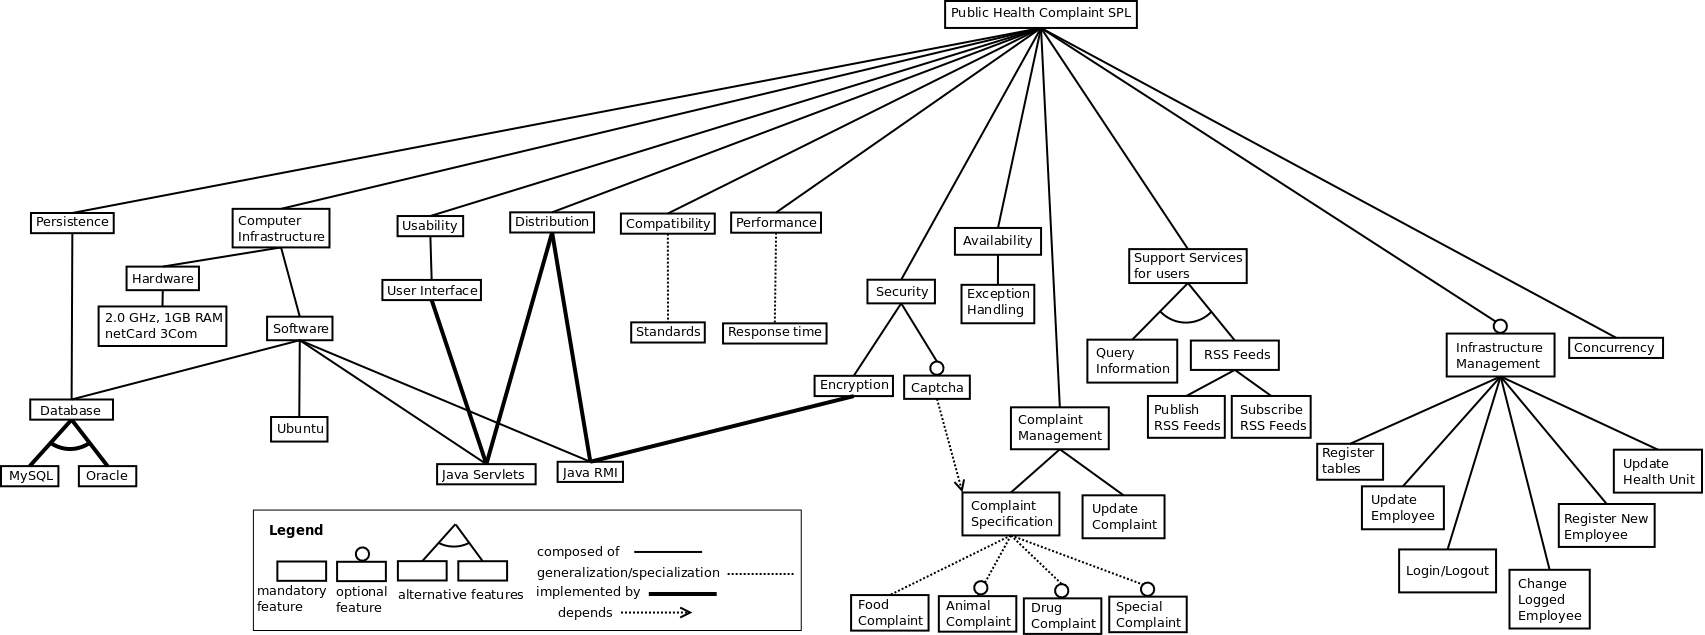
\includegraphics[scale=0.23]{figs/phs-featuremodel-v02.png}
}
   \caption{Public Health Complaint Software Product Line feature diagram}
   \label{fig:featureDiag}
\end{figure}



\subsubsection{Product Features}
\label{sec:productfeat}
It should be possible to derive three software products from the core assets of the Public Health Complaint SPL:
Healthwatcher~\cite{hw-tao},
Medwatch~\cite{medwatch}, and DPH-LA~\cite{dphla}.

Table~\ref{tab:featOfEachProd} describes the feature of each product. The creation of this table was based on use case
specification (Section~\ref{sec:useCases}). Some features were also extracted by using these software products (i.e. applications).

\begin{table}

\begin{center}
\begin{footnotesize}
\begin{tabular}{c|c|c|c} \hline
         & \multicolumn{3}{c}{\textbf{Products}}  \\ \cline{2-4}
\textbf{Features} & \textbf{Healthwatcher} & \textbf{Medwatcher} & \textbf{Environmentwatcher} \\ \hline
Public Health Complaint SPL     & \checkmark & \checkmark & \checkmark \\ \hline
Infrastructure Management       & \checkmark &            & \checkmark \\ \hline
Register tables                 & \checkmark &            & \checkmark \\ \hline
Update employee                 & \checkmark &            & \checkmark \\ \hline
Register new employee           & \checkmark &            & \checkmark \\ \hline
Change logged employee          & \checkmark &            & \checkmark \\ \hline
Login/Logout                    & \checkmark &            & \checkmark \\ \hline
Update Health Unit              & \checkmark &            & \checkmark \\ \hline
Complaint Management            & \checkmark & \checkmark & \checkmark \\ \hline
Update Complaint                & \checkmark &            & \checkmark \\ \hline
Complaint Specification         & \checkmark & \checkmark & \checkmark \\ \hline
Food Complaint Specification    & \checkmark & \checkmark & \checkmark \\ \hline
Animal Complaint Specification  & \checkmark &            & \checkmark \\ \hline
Drug Complaint Specification    &            & \checkmark &            \\ \hline
Special Complaint Specification & \checkmark &            & \checkmark \\ \hline
Support services for users      & \checkmark & \checkmark & \checkmark \\ \hline
Query Information               & \checkmark & 		  &            \\ \hline
RSS feeds			&            & \checkmark & \checkmark \\ \hline
Publish RSS feeds    		&            & \checkmark & \checkmark \\ \hline
Receive alerts via feeds	&            & \checkmark & \checkmark \\ \hline
Exception Handling 		& \checkmark & \checkmark & \checkmark \\ \hline
Security 			& \checkmark & \checkmark & \checkmark \\ \hline
Captcha                         &            &            & \checkmark \\ \hline
Encryption 			& \checkmark & \checkmark & \checkmark \\ \hline
Computer infrastructure         & \checkmark & \checkmark & \checkmark \\ \hline
Hardware                        & \checkmark & \checkmark & \checkmark \\ \hline
2.0 GHz, 1GB RAM, netCard 3Com  & \checkmark & \checkmark & \checkmark \\ \hline
Software                        & \checkmark & \checkmark & \checkmark \\ \hline
Ubuntu 10.4                     & \checkmark & \checkmark & \checkmark \\ \hline
Database                        & \checkmark & \checkmark & \checkmark \\ \hline
MySQL	                        & \checkmark & \checkmark &            \\ \hline
Oracle	                        &            &            & \checkmark \\ \hline
Java Servlets                   & \checkmark & \checkmark & \checkmark \\ \hline
Java RMI	                & \checkmark & \checkmark & \checkmark \\ \hline
Distribution                    & \checkmark & \checkmark & \checkmark \\ \hline
Usability                       & \checkmark & \checkmark & \checkmark \\ \hline
User interface                  & \checkmark & \checkmark & \checkmark \\ \hline
Compatibility                   & \checkmark & \checkmark & \checkmark \\ \hline
Standards                       & \checkmark & \checkmark & \checkmark \\ \hline
Performance                     & \checkmark & \checkmark & \checkmark \\ \hline
Response time                   & \checkmark & \checkmark & \checkmark \\ \hline
Persistence                     & \checkmark & \checkmark & \checkmark \\ \hline
Concurrency                     & \checkmark & \checkmark & \checkmark \\ \hline
\end{tabular}
\end{footnotesize}
\end{center}
\caption{Features of each product} 
\label{tab:featOfEachProd}
\end{table}

 



\subsubsection{Feature Groups}
\label{sec:featGroups}
Features can be grouped in order to place a constraint on how the features are used by a certain product~\cite{Gomaa:2004:DSP}. Establishing
these relationships among features also support building a modular product line architecture (PLA)~\cite{Lee:2004:FDA}. According to PLUS
method~\cite[Chapter 5.5]{Gomaa:2004:DSP}, there are four types of feature groups, namely \textit{exactly-one-of}, \textit{zero-or-one-of},
\textit{at-least-one-of}, \textit{zero-or-more-of}.  Table~\ref{tab:featureGroup} describes feature groups and provides additional
information about the relationship among features. 
\begin{table}
\begin{center}
\begin{footnotesize}
\begin{tabular}{c|c|c|c} \hline
 \textbf{Feature Group} & \textbf{Feature Group} & \textbf{Features in Feature} & \textbf{Feature} \\
  \textbf{Name} 	       & \textbf{Category}      & \textbf{Group}               & \textbf{Category} \\ \hline
Complaint Specification & at-least-one-of & Animal Complaint & optional \\ 
		        &              & Food Complaint & mandatory \\
			&              & Drug Complaint & optional \\
			&              & Special Complaint & optional \\  \hline
Database                & exactly-one-of  & MySQL & alternative \\
		        &                 & Oracle & alternative \\ \hline
Support services for    & at-least-one-of & Query information & alternative \\
users		        &                 & RSS feeds & alternative \\  \hline		        
\end{tabular}
\end{footnotesize}
\end{center}
\caption{Feature groups} 
\label{tab:featureGroup}
\end{table}



\section{Analysis}
\label{sec:analysis}

Figure~\ref{fig:analysis} shows that in this approach Analysis consists of three activities: \textit{Use case specification},
\textit{Croscutting concerns identification and composition}, and \textit{Aspect-oriented feature view}.


\begin{figure}[!htb]
   \centering
   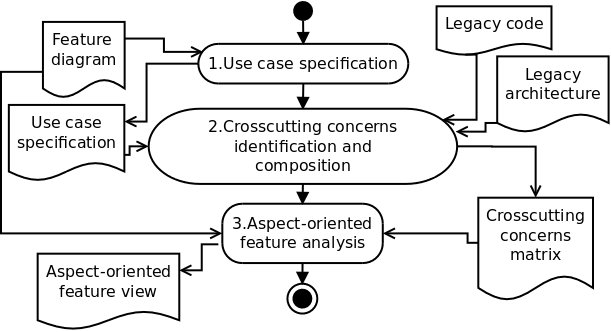
\includegraphics[scale=0.28]{figs/analysis-v01.png}
   \caption{Analysis activities}
   \label{fig:analysis}
\end{figure}

\subsection{Nonfunctional requirements}

Based on the documentation and use of the applications, we identified the nonfunctional requirements (i.e. quality attributes)
described below. The descriptions of nonfunctional requirements were either copied or adapted from Healthwatcher
Requirements~\cite{hw-usecase}, Aspect-oriented Requirements Engineering (AORE) models~\cite{hw-aore}, AORE
viewpoints~\cite{hw-viewpoints-v2}, and Multi-dimensional Separation of Concerns (MDSOC)~\cite{hw-mdsoc}.

\subsubsection{Usability [NFR01]}

\textbf{Priority:} Important

The system should have an easy to use GUI, as any person who has access to the internet should be able to use the system~\cite{hw-usecase}.
The user interface must be implemented using
Servlets~\cite{hw-usecase}.

\subsubsection{Availability/Exception Handling [NFR02]}

\textbf{Priority:} Essential


The system should be available 24 hours a day, 7 days a week. The nature of the system not being a critical system, the system might stay
off until any fault is fixed~\cite{hw-usecase}. Several functionalities might raise errors while the user interacts with the system and
require different handling techniques. General errors that apply to most cases are due to missing information (e.g. users do not fill in the
required fields in an entry form) and the system signals the error and show which fields need to be provided. Other error might be related
to entering invalid data and the error handling mechanism should try either to avoid that or to raise the error and suggest the
correction~\cite{hw-aore}. According to Bass et al.~\cite[Chapter 4.1]{Bass:1998:SAP}, availability is closely related to reliability and
one technique to improve reliability is exception handling.


\subsubsection{Performance/Response time [NFR03]}

\textbf{Priority:} Essential

The system must be capable to handle 20 simultaneous users. The response time must not exceed 5
seconds~\cite{hw-usecase,hw-alignment}.

\subsubsection{Encryption/Security [NFR04]}

\textbf{Priority:} Important

The system should use a security protocol when sending data over the internet. To have access to the complaint registration features, access
must be allowed by the access control sub-system~\cite{hw-aore,hw-usecase}.

\subsubsection{Standards/Compatibility [NFR05]}

\textbf{Priority:} Important

The system must be developed according to the standards established by X\footnote{The company name is confidential due to commercial
reasons}, responsible for the norms and standardization of systems for
the City Hall~\cite{hw-usecase,hw-alignment}.


\subsubsection{Harware and Software/Operational environment [NFR06]}

This section lists the hardware and software to be used for the system to operate in a desirable fashion~\cite{hw-usecase}.

\textbf{Software:} Ubuntu 10.04 LTS for the workstation.

\textbf{Hardware:} One computer with: 2.0 GHz processor, 1 GB of RAM memory, net card 3Com 10/100. This equipment shall be used by
the attendant as a workstation.


\subsubsection{Distribution [NFR07]}

\textbf{Priority:} Essential

The system should be capable of running on separate machines. For example, the system core could be running on one machine and the Servlets
on another~\cite{hw-usecase}.



\subsubsection{(Flexible) Storage medium/Persistence [NFR08]}

\textbf{Priority:} Essential


The persistence mechanism should store data about the complaints, employees, health units, deceases, specialities
and citizens that complaint. The system must be capable of extension on the storage matter, making possible to use, arrays
or different databases (MySQL, Oracle, etc.)~\cite{hw-aore,hw-usecase}.





\subsubsection{Concurrency [NFR09]}
\textbf{Priority:} Essential

The system must be capable to handle 20 simultaneous users~\cite{hw-aore}.


\subsection{Use cases specification}
\label{sec:useCases}

The use case specification has three main goals: (i) further detail the requirements based on legacy documentation (ii) specify use case
variability (iii) identify crosscutting and non-crosscutting use cases. In order to achieve the first goal, we elicited the use
cases based on existing documents of legacy applications. Fantechi et al. proposed an approach to use legacy requirements
document to specify product line variability~\cite{Fantechi:2004:EUC}. Even the use of legacy applications can be useful to understand them. 
Use case variability is determined based on features variability, which has already been specified in the feature diagram. PLUS
method~\cite{Gomaa:2004:DSP} represents the use case variability with stereotypes (kernel, alternative, and optional). Use cases can also represent
crosscutting concerns as proposed Jacobson and Ng~\cite[Chapter 6.2]{Jacobson:2004:ASD}. Crosscutting concerns are
represented by use case extensions, which add new behavior to the existing use cases. In this way, both variability and crosscutting concerns are
represented.

\subsubsection{Functional Use Cases}

Figure~\ref{fig:usecase} shows the use case diagram for the Public Health Complaint SPL. All use cases were adapted from \textit{Healthwatcher -
Requirements} document~\cite{hw-usecase}, but the UC05, UC15, UC16 use cases, that were included based on the domain analysis
(Section~\ref{sec:domainAnalysis}).

%TODO esta faltando o caso de uso de publicar feeds
\begin{figure}[h!t!b!]
   \centering
   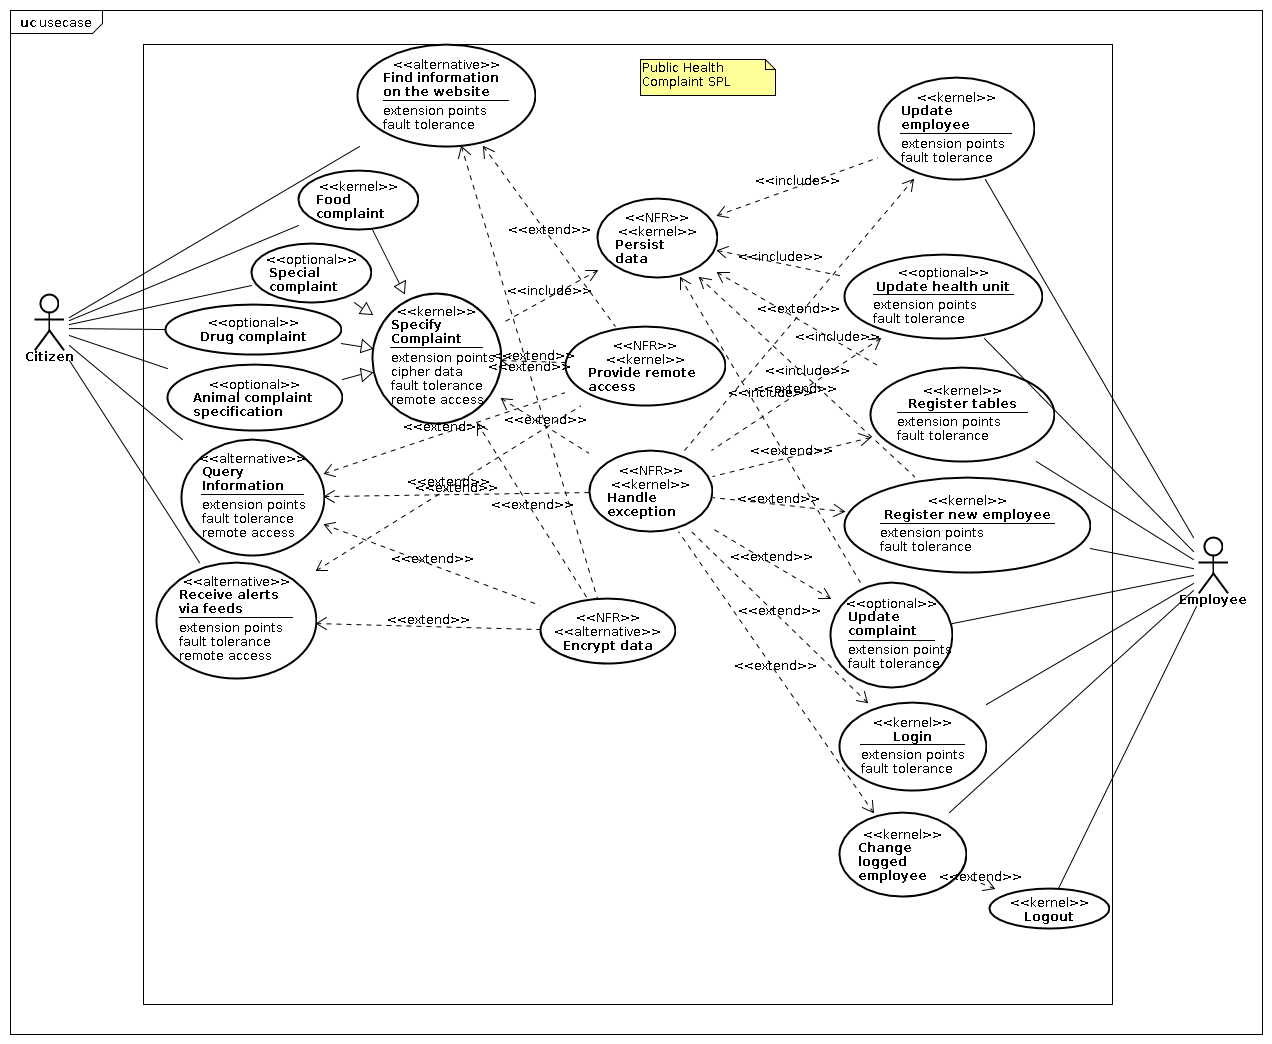
\includegraphics[scale=0.4]{figs/hw-usecase.png}
   \caption{Public Health Complaint SPL use case diagram}
   \label{fig:usecase}
\end{figure}


\textbf{Query information [UC01]}\\
\textbf{Use Case Name:} Query information\\
\textbf{Description:} This use case allows a citizen to perform queries.

\textit{Query Health Guide.} The citizen might query:
\begin{itemize}
\item Which health units take care of a specific specialty.
\item What are the specialties of a particular health unit.
\end{itemize}

\textit{Query Speciality Information.} The citizen might query:
\begin{itemize}
\item Information about a complaint made by a citizen:
\begin{itemize}
\item Complaint details.
\item Situation (OPENED, SUSPENDED, or CLOSED).
\item Technical analysis.
\item Analysis date.
\item Employee that made the analysis.
\end{itemize}
\item Information about diseases:
\begin{itemize}
\item Description.
\item Symptoms.
\item Duration.
\end{itemize}
\end{itemize}
\textbf{Priority:} Important \\ 
\textbf{Category:} Optional \\ 
\textbf{Inputs and pre-conditions:} The data to be queried must be registered on the system\\ 
\textbf{Outputs and post-conditions:}  The query result to the citizen\\  
\textbf{Main flow of events:}\\
\begin{enumerate}
\item \label{uc01:exc01}The citizen chooses the type of query
\begin{enumerate}
\item  In the case of query on specialties grouped by health units, the
system retrieves the list of health units stored.
\begin{enumerate}
 \item The system retrieves the details of each health unit such as its
description and specialties.
\item The list of health units is presented to the user on their local
display. 
\end{enumerate}
\item In the case of a query on health units grouped by specialties, the
system retrieves the list of registered specialties. 
\begin{enumerate}
\item The system retrieves the details of each specialty such as its
unique identifier and name.
\item The list of specialties is presented to the user on their local
display.
\end{enumerate}
\item In the case of a query on diseases, the system retrieves the list of
diseases.
\begin{enumerate}
\item The system retrieves the details of each disease type such as
its unique identifier and name.
\item The list of disease is presented to the user on their local
display. 
\end{enumerate}
\end{enumerate}
\item \label{uc01:exc02} The citizen provides the data for the query
\begin{enumerate}
\item In the case of a query on specialties grouped by health units, the
citizen selects the health unit to be queried.
\begin{enumerate}
\item A unique identifier representing the selected health unit is sent
to the server.
\item The system ensures the health unit information is consistent.
\item The unique identifier is used by the system to search the
repository for the selected health unit.
\item The details of the selected health unit are retrieved including its
specialties.
\item The specialties for the selected health unit are returned to the
user.
\end{enumerate}
\item In the case of a query on health units grouped by specialties, the
citizen selects the specialty to be queried.
\begin{enumerate}
\item A unique identifier representing the selected specialty is sent to
the server.
\item The system ensures the health unit information is consistent.
\item The unique identifier is used to retrieve the list of health units
which are associated with the selected specialty.
\item The details of the health units and specialties are retrieved.
\item The retrieved health units are returned to the user.
\end{enumerate}
\item In the case of a query on complaints, the citizen provides the
complaint code.
\begin{enumerate}
\item The unique identifier representing the complaint to be retrieved
is sent to the server.
\item The system ensures the complaint information is consistent.
\item The unique identifier is used to retrieve the complaint entry.
\item The system must determine the complaint type as to retrieve
the appropriate information.
\begin{enumerate}
\item If the complaint is a special complaint the complainer's
age, education level and occupation are retrieved (in
addition to the standard complaint information).
\item If the complaint is a food complaint the meal which was
consumed, the number of people who ate the meal, the
number of sick people, etc. are retrieved (in addition to
the standard complaint information).
\item If the complaint is an animal complaint the animal
species and the number of animals affected (in addition
to the standard complaint information).
\end{enumerate}
\item The complaint with all the appropriate information is returned to
the user.
\end{enumerate}
\item In the case of a query on diseases, the citizen selects the disease to
be queried.
\begin{enumerate}
\item The unique identifier is used to retrieve the list of health units
which are associated with the selected specialty.
\item The details of the health units and specialties are retrieved.
\item The retrieved health units are returned to the user.
\end{enumerate}
\item In the case of a query on complaints, the citizen provides the
complaint code.
\begin{enumerate}
\item The unique identifier representing the complaint to be retrieved
is sent to the server.
\item The system ensures the complaint information is consistent.
\item The unique identifier is used to retrieve the complaint entry.
\item The system must determine the complaint type as to retrieve
the appropriate information.
\begin{enumerate}
\item If the complaint is a special complaint the complainer's
age, education level and occupation are retrieved (in
addition to the standard complaint information).
\item If the complaint is a food complaint the meal which was
consumed, the number of people who ate the meal, the
number of sick people, etc. are retrieved (in addition to
the standard complaint information).
\item If the complaint is an animal complaint the animal
species and the number of animals affected (in addition
to the standard complaint information).
\end{enumerate}
\item The complaint with all the appropriate information is returned to
the user.
\end{enumerate}
\item In the case of a query on diseases, the citizen selects the disease to
be queried.
\begin{enumerate}
\item The unique identifier representing the disease type to be
retrieved is sent to the server.
\item The system ensures the disease type information is consistent.
\item The unique identifier is used to retrieve the disease type to
query.
\item The symptoms for the selected disease type are retrieved.
\item The complete disease information is returned to the user.
\end{enumerate}
\end{enumerate}
\item The query results are formatted and presented to the user on their local display.
\end{enumerate}

% \textbf{Extension Points:}\\
% \textbf{E1. Send data over the internet}\\
% The \textit{Send data over the internet} extension point occurs before step~\ref{uc01:ep01}

\textbf{Specify complaint [UC02]}\\
\textbf{Use Case Name:} Specify complaint\\
\textbf{Description:} This use case allows a citizen to register complaints. Complaints can be related to Food, Animal, Drugs, or
Special. The four kinds of complaints have the following information in common: Complaint data: description (mandatory) and observations
(optional);\\
\textbf{Priority:} Essential \\ 
\textbf{Category:} Optional \\ 
\textbf{Inputs and pre-conditions:} None\\ 
\textbf{Outputs and post-conditions:}  The complaint saved on the system\\  
\textbf{Main flow of events:}\\
\begin{enumerate}
\item The citizen selects the kind of complaint.
\item The system shows the specific screen for each type of complaint.
\item The system registers the kind, date and time of the complaints.
\item The citizen provides the complaint specific data.
\item \label{uc02:ep01}The system saves the complaint.
\begin{enumerate}
\item The information entered by the user is sent to the server.
\item The system parses the data entered by the user.
\item The system creates a new instance of the appropriate complaint
type.
\item The system generates a unique identifier and assigns this to the new
complaint.
\item The complainers address is parsed and saved.
\item The common complaint information is parsed and stored with the
OPENED state.
\item The specific complaint data is then extracted and stored accordingly.
\item The system ensures the data is left in a consistent state.
\end{enumerate}
\item The unique identifier is returned and presented to the user on their local
display.
\end{enumerate}

\textbf{Extension Points:}\\
\textbf{E1. Send data over the internet}\\
The \textit{Send data over the internet} extension point occurs before step~\ref{uc02:ep01}


\textbf{Food complaint specification [UC03]}\\
\textbf{Use Case Name:} Food complaint specification\\
\textbf{Description:} 
Food Complaint - DVISA
\begin{itemize}
\item Cases where there is a suspicion infected food being eaten.
\end{itemize}
\textbf{Priority:} Essential\\
\textbf{Category:} Mandatory\\
\textbf{Inputs and pre-conditions:} none\\
\textbf{Outputs and post-conditions:} The food complaint is saved on the system\\
\textbf{Main flow of events:}\\
\begin{enumerate}
\item The citizen chooses \textit{Food} as the kind of complaint.
\item The system shows the \textit{Food} complaint screen.
\item The system registers the kind, date and time of the complaints.
\item The citizen provides the complaint specific data.
\item The system saves the complaint.
\begin{enumerate}
\item The information entered by the user is sent to the server.
\item The system parses the data entered by the user.
\item The system creates a new instance of the appropriate complaint
type.
\item The system generates a unique identifier and assigns this to the new
complaint.
\item The complainers address is parsed and saved.
\item The common complaint information is parsed and stored with the
OPENED state.
\item The specific complaint data is then extracted and stored accordingly.
\item The system ensures the data is left in a consistent state.
\end{enumerate}
\item The unique identifier is returned and presented to the user on their local
display.
\end{enumerate}

\textbf{Animal complaint specification [UC04]}\\
\textbf{Use Case Name:} Animal complaint specification \\
\textbf{Description:} This use case allows a citizen to register food complaints\\
Animal Complaint - DVA
\begin{itemize}
\item Sick animals.
\item Infestations (rodents, scorpions, bats, etc.)
\item Diseases related to mosquitoes (dengue, filariose).
\item Animal maltreatment
\end{itemize}
\textbf{Priority:} Essential \\
\textbf{Category:} Optional \\
\textbf{Inputs and pre-conditions:} none\\
\textbf{Outputs and post-conditions:}The animal complaint is saved on the system\\
\textbf{Main flow of events:}\\
\begin{enumerate}
\item The citizen chooses \textit{Animal} as the kind of complaint.
\item The system shows the \textit{Animal} complaint screen.
\item The system registers the kind, date and time of the complaints.
\item The citizen provides the complaint specific data.
\item The system saves the complaint.
\begin{enumerate}
\item The information entered by the user is sent to the server.
\item The system parses the data entered by the user.
\item The system creates a new instance of the appropriate complaint
type.
\item The system generates a unique identifier and assigns this to the new
complaint.
\item The complainers address is parsed and saved.
\item The common complaint information is parsed and stored with the
OPENED state.
\item The specific complaint data is then extracted and stored accordingly.
\item The system ensures the data is left in a consistent state.
\end{enumerate}
\item The unique identifier is returned and presented to the user on their local
display.
\end{enumerate}

\textbf{Drug complaint specification [UC05]}\\
\textbf{Use Case Name:} Drug complaint specification\\
\textbf{Description:}
Required information for a drug complaint: 
\begin{itemize}
\item Patient information: Patient identifier; patient age; patient weight in kilograms or pounds
\item Type of problem (check at least one of the following): Adverse event; Product use error; Product problem (e.g. defects, malfunction);
Problem with different manufacturer of same medicine
\item Outcomes attributed to adverse event (check at least one of the following): Death (specify the date); Life-threatening;
Hospitalization - initial or prolonged; Disability or permanent damage; Congenital anomaly/Birth defect; Required intervention to prevent
permanent impairment/damage (devices); Other serious (important medical events)
\item Date of event 
\item Date of this complaint (automatically filled)
\item Describe the event, problem or use error textually (up to a total of 6400 characters allowed.)
\item Relevant tests/Laboratory data, including dates (textual description up to a total of 2000 characters allowed.)
\item Other Relevant History, Including Preexisting Medical Conditions (e.g. allergies, race, pregnancy, smoking and alcohol use,
liver/kidney problems,etc.) Textual description up to a total of 2000 characters allowed.
\item Product Available for Evaluation (check one of the following): yes, no, returned to the manufacturer on (specify the date)
\item Suspected products information: Product name; Label strength; manufacturer/labeler; dose/amount; frequency; route; dates of use (If
unknown, give duration) from/to (or best estimate); Diagnosis or Reason for Use (Indication); Event Abated After Use Stopped or Dose
Reduced? (check one of the following): yes, no, doesn't apply; lot number; expiration date; Event Reappeared After Reintroduction? (check
one of the following): yes, no, doesn't apply; NDC number or Unique ID.
\item Suspected medical device: brand name; common device name; manufacturer name, city, and state; model number; catalog number; serial
number; lot number; expiration date; other number; operator device (check one of the following): health professional, lay user/patient,
other (specify); if implanted, give date; if explanted, give date; is this a single use device that was reprocessed and reused on a
patient? (check one of the following): yes, no; if yes to previous item, enter name and address of reprocessor (textual description up to a
total of 450 characters allowed)
\item  Product names and therapy dates (exclude treatment of event). Up to a total of 2000 characters allowed 
\item Reporter information: name; address; city; state; zip code; phone number; email; health professional (check one of the following):
yes, no; also reported to (check as many as you want): manufacturer, user facility, distributor/importer;  If you do NOT want your identity
disclosed to the manufacturer, check here (checkbox)  
\end{itemize}
\textbf{Priority:} Essential \\ 
\textbf{Category:} Optional \\ 
\textbf{Inputs and pre-conditions:} None\\ 
\textbf{Outputs and post-conditions:}  The drug complaint is saved on the system\\  
\textbf{Main flow of events:}\\
\begin{enumerate}
\item The citizen chooses \textit{Drug} as the kind of complaint.
\item The system shows the \textit{Drug} complaint screen.
\item The system registers the kind, date and time of the complaints.
\item The citizen provides the complaint specific data.
\item The system saves the complaint.
\begin{enumerate}
\item The information entered by the user is sent to the server.
\item The system parses the data entered by the user.
\item The system creates a new instance of the appropriate complaint
type.
\item The system generates a unique identifier and assigns this to the new
complaint.
\item The complainers address is parsed and saved.
\item The common complaint information is parsed and stored with the
OPENED state.
\item The specific complaint data is then extracted and stored accordingly.
\item The system ensures the data is left in a consistent state.
\end{enumerate}
\item The unique identifier is returned and presented to the user on their local
display.
\end{enumerate}



\textbf{Special complaint specification [UC06]}\\
\textbf{Use Case Name:} Special complaint specification \\
\textbf{Description:} Special Complaint - DVISA
\begin{itemize}
 \item Cases related to several reasons, which are not mentioned above
(restaurants with hygiene problems, leaking sewerage, suspicious
water transporting trucks, etc.)
\end{itemize}
\textbf{Priority:} Essential\\
\textbf{Category:} Optional\\
\textbf{Inputs and pre-conditions:} none\\
\textbf{Outputs and post-conditions:}  The drug complaint is saved on the system\\
\textbf{Main flow of events:}\\
\begin{enumerate}
\item The citizen chooses \textit{Special} as the kind of complaint.
\item The system shows the \textit{Special} complaint screen.
\item The system registers the kind, date and time of the complaints.
\item The citizen provides the complaint specific data.
\item The system saves the complaint.
\begin{enumerate}
\item The information entered by the user is sent to the server.
\item The system parses the data entered by the user.
\item The system creates a new instance of the appropriate complaint
type.
\item The system generates a unique identifier and assigns this to the new
complaint.
\item The complainers address is parsed and saved.
\item The common complaint information is parsed and stored with the
OPENED state.
\item The specific complaint data is then extracted and stored accordingly.
\item The system ensures the data is left in a consistent state.
\end{enumerate}
\item The unique identifier is returned and presented to the user on their local
display.\end{enumerate}

\textbf{Login [UC07]}\\
\textbf{Use Case Name:} Login\\
\textbf{Description:} This use case allows an employee to have access to restricted operations on
the Health-Watcher system.\\
\textbf{Priority:} Essential \\ 
\textbf{Category:} Optional \\ 
\textbf{Inputs and pre-conditions:} None\\ 
\textbf{Outputs and post-conditions:} Password validated by the system\\  
\textbf{Main flow of events:}\\
\begin{enumerate}
\item The employee provides the login and password.
\item \label{uc07:ep01}The login and password are sent to the server.
\item The system retrieves the employee details using the login as a unique
identifier.
\item The system validates the entered password.
\item The result of the login attempt is presented to the employee on their
local display.
\end{enumerate}

\textbf{Extension Points:}\\
\textbf{E1. Send data over the internet}\\
The \textit{Send data over the internet} extension point occurs before step~\ref{uc07:ep01}


\textbf{Logout [UC08]}\\
\textbf{Use Case Name:} Logout\\
\textbf{Description:} The employee logouts the system\\
\textbf{Priority:} Essential \\ 
\textbf{Category:} Optional \\ 
\textbf{Inputs and pre-conditions:} The employee is logged in\\ 
\textbf{Outputs and post-conditions:}  The employee is not logged in\\  
\textbf{Main flow of events:}\\
\begin{enumerate}
\item The employee clicks on \textit{Logout} button
\item The system logs out the employee
\end{enumerate}



\textbf{Register tables [UC09]}\\
\textbf{Use Case Name:} Register tables\\
\textbf{Description:} This use case allows the registration of system tables. The following operations are possible: insert, update, delete,
search and print. The available tables include:\\
\begin{itemize}
\item Health unit (unit code, unit description).
\item Specialty (code and description).
\item Health unit / Specialty (health unit and specialty).
\item Employee (login, name and password).
\item Type of disease (code, name, description, symptom and duration).
\item Symptom (code and description).
\item Type of disease / Symptom (type of disease and symptom).
\end{itemize}
\textbf{Priority:} Essential\\
\textbf{Category:} \\
\textbf{Inputs and pre-conditions:} Verified employees\\
\textbf{Outputs and post-conditions:} Updated data on tables\\
\textbf{Main flow of events:}\\
\begin{enumerate}
\item The employee chooses the option to register (insert/update) in one of the tables.
\item The employee enters the data.
\item\label{uc09:ep01} The system saves the data.
\end{enumerate}


\textbf{Extension Points:}\\
\textbf{E1. Send data over the internet}\\
The \textit{Send data over the internet} extension point occurs before step~\ref{uc09:ep01}

\textbf{Update complaint [UC10]}\\
\textbf{Use Case Name:} Update complaint \\
\textbf{Description:} This use case allows the state of a complaint to be updated.\\
\textbf{Priority:} Essential\\
\textbf{Category:} Mandatory\\
\textbf{Inputs and pre-conditions:} 
\begin{itemize}
\item The complaint must be registered and have the OPENED state.
\item Verified employee
\end{itemize}
\textbf{Outputs and post-conditions:} Complaint updated and with state CLOSED.\\
\textbf{Main flow of events:}\\
\begin{enumerate}
\item The employee selects the update complaint option.
\item The system retrieves the list of all registered complaints.
\begin{enumerate}
\item The complaint list is populated with general and complaint type
specific data.
\end{enumerate}
\item The list of complaints is returned to the employee.
\item The complaints are formatted and presented to the employee on their
local display.
\item \label{uc10:ep01a}The employee selects the complaint they wish to update.
\item The complaint unique identifier is sent to the server.
\item The system ensures the complaint data is consistent.
\item The system retrieves the complaint entry.
\item The complaint is returned to the employee.
\item The complaint is formatted and presented to the employee on their local
display.
\item The employee enters the conclusion.
\item \label{uc10:ep01b}The conclusion is sent to the server.
\item The complaint status is set to closed; the date the conclusion was entered
is set in addition to the employee who dealt with the complaint.
\item The system ensures the complaint is left in a consistent state.
\item The complaint information is updated to store the new information.
\end{enumerate}

\textbf{Extension Points:}\\
\textbf{E1. Send data over the internet}\\
The \textit{Send data over the internet} extension point occurs before steps~\ref{uc10:ep01a} and \ref{uc10:ep01b}

\textbf{Register new employee [UC11]}\\
\textbf{Use Case Name:} Register new employee \\
\textbf{Description:} This use case allows new employees to be registered on the system.\\
\textbf{Priority:} Essential \\
\textbf{Category:} Mandatory \\
\textbf{Inputs and pre-conditions:} Verified employee\\
\textbf{Outputs and post-conditions:}New employee registered on the system\\
\textbf{Main flow of events:}\\
\begin{enumerate}
\item The employee selects the insert employee option.
\item The employee provides the following information about the new
employee: Name, Login ID, Password (with second password field for confirmation).
\item The employee confirms the operation.
\item \label{uc11:ep01} The entered data is transmitted to the server.
\item The system verifies the entered data.
\item The system ensures employee data is consistent.
\item The system saves the new employee's data.
\end{enumerate}

\textbf{Extension Points:}\\
\textbf{E1. Send data over the internet}\\
The \textit{Send data over the internet} extension point occurs before step~\ref{uc11:ep01}

\textbf{Update employee [UC12]}\\
\textbf{Use Case Name:} Update employee\\
\textbf{Description:} This use case allows of the employee's data to be updated on the system.\\
\textbf{Priority:} Essential \\
\textbf{Category:} Mandatory\\
\textbf{Inputs and pre-conditions:} Verified employee \\
\textbf{Outputs and post-conditions:} Employee's data updated on the system\\
\textbf{Main flow of events:}\\
\begin{enumerate}
\item The employee chooses the update employee option.
\item The employee provides the data to be updated: \textit{Name}, \textit{New password} (with second password field for confirmation),
\textit{Current password}
\item The employee confirms the update.
\item \label{uc12:ep01}The entered data is sent to the server.
\item The system verifies the entered data.
\item The system ensures the employee data is consistent.
\item The system stores the updated employee information.
\end{enumerate}

\textbf{Extension Points:}\\
\textbf{E1. Send data over the internet}\\
The \textit{Send data over the internet} extension point occurs before step~\ref{uc12:ep01}

\textbf{Update health unit [UC13]}\\
\textbf{Use Case Name:} Update health unit \\
\textbf{Description:} This use case allows the health unit's data to be updated.\\
\textbf{Priority:} Essential \\
\textbf{Category:} Mandatory \\
\textbf{Inputs and pre-conditions:} Verified employee \\
\textbf{Outputs and post-conditions:} Health unit's data updated on the system.\\
\textbf{Main flow of events:}\\
\begin{enumerate}
\item The employee chooses the update health unit option.
\item The system retrieves the list of all health units.
\item The list of health units is returned to the employee.
\item The list of health units is formatted and displayed on the employee's local
display.
\item  The employee selects the health unit to be updated.
\item  \label{uc13:ep01a}The unique identifier for the selected health unit is sent to the server.
\item  The system ensures the health unit data is consistent.
\item  The system retrieves the data for the selected health unit.
\item  The data retrieved is returned to the employee.
\item  The health unit data is formatted and presented on the employee's local
display.
\item  The employee alters the necessary data.
\item  \label{uc13:ep01b}The updated information is sent to the server.
\item  The system ensures the health unit data is left in a consistent state.
\item  The system stores the updated health unit information.
\end{enumerate}

\textbf{Extension Points:}\\
\textbf{E1. Send data over the internet}\\
The \textit{Send data over the internet} extension point occurs before steps~\ref{uc13:ep01a} and \ref{uc13:ep01b}

\textbf{Change logged employee [UC14]}\\
\textbf{Use Case Name:} Change logged employee\\
\textbf{Description:} This use case allows the currently logged employee to be changed.\\
\textbf{Priority:} Essential \\
\textbf{Category:} Mandatory \\
\textbf{Inputs and pre-conditions:} Verified employee \\
\textbf{Outputs and post-conditions:} First employee signed out and new employee logged-in.\\
\textbf{Main flow of events:}\\
\begin{enumerate}
\item The employee chooses the change logged employee option.
\item The system shows the login screen, and from this point on, the flow will follow the one described in [Login].\\
\end{enumerate}



\textbf{Receive alerts via feeds [UC15]}\\
\textbf{Use Case Name:} Receive alerts via feeds \\
\textbf{Priority:} Desirable  \\ 
\textbf{Category:} Optional \\ 
\textbf{Inputs and pre-conditions:} The citizen is using a browser which is capable of subscribing to feed \\ 
\textbf{Outputs and post-conditions:} The citizen receives feeds from Public Health Complaint SPL \\  
\textbf{Main flow of events:}\\
\begin{enumerate}
\item The citizen clicks on the link to subscribe to Public Health Complaint SPL feed
\item The system displays some options for the citizen to choose how to subscribe the feeds
\item The citizen selects one option
\item The system registers the citizen
\end{enumerate}

\textbf{Publish feeds [UC16]}\\
\textbf{Use Case Name:} Receive alerts via feeds \\
\textbf{Priority:} Desirable  \\ 
\textbf{Category:} Optional \\ 
\textbf{Inputs and pre-conditions:} Update complaint (UC10)\\ 
\textbf{Outputs and post-conditions:} Feeds will be updated \\  

\textbf{Main flow of events:}\\
This use case is triggered automatically after a complaint is updated by an employee [UC10]. Data related to the updated complaint is
used to create a feed entry that will be published. 

\subsubsection{Nonfunctional Use Cases}
\label{sec:nonfunctionalUsecases}
%TODO rever a frase na qual cito a Rubira. Nao tenho certeza que essa eh a referencia certa
Some nonfunctional requirements can be refined as nonfunctional use cases (also known as infrastructure use cases), such as persistence and
encryption, which are described in this
section. There are also other kinds of nonfunctional requirements that represent system wide qualities and are described simply as
declarative statements during requirements~\cite[Chapter 7.3]{Jacobson:2004:ASD}. Although exception handling is a nonfunctional requirement
and it would be possible to specify it as a nonfunctional use case, we follow the approach proposed by Rubira et al.~\cite{Rubira:2005:EHD}
and specify the exceptional behavior as use case extensions (Section~\ref{sec:ehusecases}).

\textbf{Persist Data [NUC01]}\\
\textbf{Use Case Name:} Persist data\\
\textbf{Priority:} Essential  \\ 
\textbf{Category:} Kernel \\ 
\textbf{Actor:} system\\
\textbf{Inputs and pre-conditions:} none\\ 
\textbf{Outputs and post-conditions:} data is stored on database \\  
\textbf{Extension flow of events:} none\\
\begin{enumerate}
\item The system stores the data entered by the user on the database
\end{enumerate}

\textbf{Encrypt Data [NUC02]}\\
\textbf{Use Case Name:} Encrypt data\\
\textbf{Description:} The system should use a security protocol when sending data over the internet. To have access to the complaint
registration features, access must be allowed by the access control sub-system~\cite{hw-usecase}.\\
\textbf{Priority:} Important \\ 
\textbf{Category:} Mandatory \\ 
\textbf{Actor:} system\\
\textbf{Inputs and pre-conditions:} none\\ 
\textbf{Outputs and post-conditions:} data is stored on database \\  
\textbf{Extension flow of events:}\\
This extension flow occurs at the extension points \textit{Send data over the internet} in the \textit{Query information}, 
\textit{Login}, \textit{Receive alerts via feeds}, \textit{Find information on the website}, and \textit{Specify
complaint} use cases.
\begin{enumerate}
\item The system uses a security protocol to send data over the internet 
\end{enumerate}

\textbf{Provide remote access [NUC03]}\\
\textbf{Use Case Name:} Provide remote access\\
\textbf{Priority:} Essential  \\ 
\textbf{Category:} Kernel \\ 
\textbf{Actor:} system\\
\textbf{Inputs and pre-conditions:} none\\ 
\textbf{Outputs and post-conditions:} data can be send over the Internet\\  
\textbf{Extension flow of events:} This extension flow occurs at the extension points \textit{Send data over the internet} in the
\textit{Query information}, \textit{Receive alerts via feeds}, \textit{Find information on the website}, and
\textit{Specify complaint} use cases.
\\
\begin{enumerate}
\item The system send data over the Internet.
\end{enumerate}

\subsubsection{Exception Handling Flow in Use Cases}
%TODO verificar os fluxos alternativos mostrados no documento de casos de uso
\label{sec:ehusecases}
\textbf{Query Information}
\textbf{Use Case Name:} Query Information\\
\textbf{Exceptions:}
\begin{enumerate}
 \item \textbf{Exception \#1:}
 \begin{itemize}
  \item \textbf{Description of Exception Behavior:} Problems on Internet Connection
  \item \textbf{Number of the Event that Identify the Exception:} \ref{uc01:exc01} and \ref{uc01:exc02}
  \item \textbf{Activity of Exception Handling:} Warn the user about the problem with a message
  \item \textbf{Group of valid post-conditions after the Exception:} The query won't be executed and the system won't be changed
 \end{itemize}
 \item \textbf{Exception \#2:}
 \begin{itemize}
  \item \textbf{Description of Exception Behavior:} A problem occurs retrieving data
  \item \textbf{Number of the Event that Identify the Exception:} 1.x.i, 2.x.iv
  \item \textbf{Activity of Exception Handling:} Warn the user about the problem with a message and the system retrieve the available
information
  \item \textbf{Group of valid post-conditions after the Exception:} The query won't be executed and the system won't be changed
 \end{itemize}
 \item \textbf{Exception \#3:}
 \begin{itemize}
  \item \textbf{Description of Exception Behavior:} An invalid complaint code is entered
  \item \textbf{Number of the Event that Identify the Exception:} 2.c.iii
  \item \textbf{Activity of Exception Handling:} Warn the user with a message that the number of this complaint is invalid
  \item \textbf{Group of valid post-conditions after the Exception:} The screen is showing the principal screen of Query Information
 \end{itemize}
 \item \textbf{Exception \#4:}
 \begin{itemize}
  \item \textbf{Description of Exception Behavior:} Consistent data cannot be assured
  \item \textbf{Number of the Event that Identify the Exception:} 2.x.ii
  \item \textbf{Activity of Exception Handling:} Warn the user with a message, the system abandon the retrieval
  \item \textbf{Group of valid post-conditions after the Exception:} The screen is showing the principal screen of Query Information
 \end{itemize}
\end{enumerate}

\textbf{Complaint Specification, Food Complaint, Animal Complaint, Special Complaint}
\textbf{Use Case Name:} Complaint Specification\\
\textbf{Exceptions:}
\begin{enumerate}
 \item \textbf{Exception \#1:}
 \begin{itemize}
  \item \textbf{Description of Exception Behavior:} Problems on Internet Connection
  \item \textbf{Number of the Event that Identify the Exception:} 5.a
  \item \textbf{Activity of Exception Handling:} Warn the user about the problem with a message
  \item \textbf{Group of valid post-conditions after the Exception:} The screen is back to the main screen of complaint specification
 \end{itemize}
 \item \textbf{Exception \#2:}
 \begin{itemize}
  \item \textbf{Description of Exception Behavior:} Invalid data is entered by the user
  \item \textbf{Number of the Event that Identify the Exception:} 5.b
  \item \textbf{Activity of Exception Handling:} Warn the user about the problem with a message
  \item \textbf{Group of valid post-conditions after the Exception:} The screen is back to the main screen of complaint specification
 \end{itemize}
 \item \textbf{Exception \#3:}
 \begin{itemize}
  \item \textbf{Description of Exception Behavior:} A problem occurs storing the complaint
  \item \textbf{Number of the Event that Identify the Exception:} 5.e-5.g
  \item \textbf{Activity of Exception Handling:} Warn the user about the problem with a message, and roll-back the complaint entry
  \item \textbf{Group of valid post-conditions after the Exception:} The screen is back to the main screen of complaint specification
 \end{itemize}
 \item \textbf{Exception \#4:}
 \begin{itemize}
  \item \textbf{Description of Exception Behavior:} Data Consistency cannot be ensured
  \item \textbf{Number of the Event that Identify the Exception:} 5.h
  \item \textbf{Activity of Exception Handling:} Warn the user about the problem with a message, and roll-back the complaint entry
  \item \textbf{Group of valid post-conditions after the Exception:} The screen is back to the main screen of complaint specification
 \end{itemize}
\end{enumerate}

\textbf{Login}
\textbf{Use Case Name:} Login\\
\textbf{Exceptions:}
\begin{enumerate}
 \item \textbf{Exception \#1:}
 \begin{itemize}
  \item \textbf{Description of Exception Behavior:} Problems on Internet Connection
  \item \textbf{Number of the Event that Identify the Exception:} 2
  \item \textbf{Activity of Exception Handling:} Warn the user about the problem with a message
  \item \textbf{Group of valid post-conditions after the Exception:} The screen is back to the main screen of Login
 \end{itemize}
 \item \textbf{Exception \#2:}
 \begin{itemize}
  \item \textbf{Description of Exception Behavior:} Problem when the system was retrieving the employee details
  \item \textbf{Number of the Event that Identify the Exception:} 3
  \item \textbf{Activity of Exception Handling:} Warn the user about the problem with a message
  \item \textbf{Group of valid post-conditions after the Exception:} The screen is back to the main screen of Login
 \end{itemize}
 \item \textbf{Exception \#3:}
 \begin{itemize}
  \item \textbf{Description of Exception Behavior:} The system cannot validate the employee (adapted from Healthwatcher - Use cases
specification~\cite{hw-usecase})
  \item \textbf{Number of the Event that Identify the Exception:} 3
  \item \textbf{Activity of Exception Handling:} Warn the user about the problem with a message
  \item \textbf{Group of valid post-conditions after the Exception:} The screen is back to the main screen of Login
 \end{itemize}
\end{enumerate}

\textbf{Register Tables}
\textbf{Use Case Name:} Register Tables\\
\textbf{Exceptions:}
\begin{enumerate}
 \item \textbf{Exception \#1:}
 \begin{itemize}
  \item \textbf{Description of Exception Behavior:} Problems on Internet Connection
  \item \textbf{Number of the Event that Identify the Exception:} 5.a
  \item \textbf{Activity of Exception Handling:} Warn the user about the problem with a message
  \item \textbf{Group of valid post-conditions after the Exception:} The screen is back to the main screen of complaint specification
 \end{itemize}
 \item \textbf{Exception \#2:}
 \begin{itemize}
  \item \textbf{Description of Exception Behavior:} Invalid data is entered by the user
  \item \textbf{Number of the Event that Identify the Exception:} 5.b
  \item \textbf{Activity of Exception Handling:} Warn the user about the problem with a message
  \item \textbf{Group of valid post-conditions after the Exception:} The screen is back to the main screen of complaint specification
 \end{itemize}
\end{enumerate}

\textbf{Update Complaint}
\textbf{Use Case Name:} Update Complaint\\
\textbf{Exceptions:}
\begin{enumerate}
 \item \textbf{Exception \#1:}
 \begin{itemize}
  \item \textbf{Description of Exception Behavior:} Error during the retrieve of registered complaints
  \item \textbf{Number of the Event that Identify the Exception:} 2, 8
  \item \textbf{Activity of Exception Handling:} Warn the user about the problem with a message
  \item \textbf{Group of valid post-conditions after the Exception:} The screen is back to the main screen of update complaint
 \end{itemize}
 \item \textbf{Exception \#2:}
 \begin{itemize}
  \item \textbf{Description of Exception Behavior:} Data consistency cannot be ensured
  \item \textbf{Number of the Event that Identify the Exception:} 7, 14
  \item \textbf{Activity of Exception Handling:} Warn the user about the problem with a message, and roll-back the complaint entry
  \item \textbf{Group of valid post-conditions after the Exception:} The screen is back to the main screen of complaint specification
 \end{itemize}
 \item \textbf{Exception \#3:}
 \begin{itemize}
  \item \textbf{Description of Exception Behavior:} Problems on Internet Connection
  \item \textbf{Number of the Event that Identify the Exception:} 3, 6, 9, 12
  \item \textbf{Activity of Exception Handling:} Warn the user about the problem with a message
  \item \textbf{Group of valid post-conditions after the Exception:} The screen is back to the main screen of update complaint
 \end{itemize}
 \item \textbf{Exception \#4:}
 \begin{itemize}
  \item \textbf{Description of Exception Behavior:} Error during the update of complaint
  \item \textbf{Number of the Event that Identify the Exception:} 15
  \item \textbf{Activity of Exception Handling:} Warn the user about the problem with a message, and roll-back the complaint entry
  \item \textbf{Group of valid post-conditions after the Exception:} The screen is back to the main screen of update complaint
 \end{itemize}
\end{enumerate}

\textbf{Register New Employee}
\textbf{Use Case Name:} Register New Employee\\
\textbf{Exceptions:}
\begin{enumerate}
 \item \textbf{Exception \#1}
 \begin{itemize}
  \item \textbf{Description of Exception Behavior:} Incomplete Data Entry (adapted from Healthwatcher - Use cases
specification~\cite{hw-usecase})
  \item \textbf{Number of the Event that Identify the Exception:} 2
  \item \textbf{Activity of Exception Handling:} Warn the user that he/she has missing/incorrect data
  \item \textbf{Group of valid post-conditions after the Exception:} The screen is back to the main screen of Register New Employee
 \end{itemize}
 \item \textbf{Exception \#2}
 \begin{itemize}
  \item \textbf{Description of Exception Behavior:} Problems on Internet Connection
  \item \textbf{Number of the Event that Identify the Exception:} 4
  \item \textbf{Activity of Exception Handling:} Warn the user about the problem with a message
  \item \textbf{Group of valid post-conditions after the Exception:} The screen is back to the main screen of Register New Employee
 \end{itemize}
 \item \textbf{Exception \#3}
 \begin{itemize}
  \item \textbf{Description of Exception Behavior:} The Employee is already entry
  \item \textbf{Number of the Event that Identify the Exception:} 5
  \item \textbf{Activity of Exception Handling:} Warn the user that already has this employee subscribed on the system and abandon the entry
  \item \textbf{Group of valid post-conditions after the Exception:} The screen is back to the main screen of Register New Employee
 \end{itemize}
 \item \textbf{Exception \#4}
 \begin{itemize}
  \item \textbf{Description of Exception Behavior:} Data consistency cannot be ensured
  \item \textbf{Number of the Event that Identify the Exception:} 6
  \item \textbf{Activity of Exception Handling:} Warn the user about the problem with a message, and roll-back the complaint entry
  \item \textbf{Group of valid post-conditions after the Exception:} The screen is back to the main screen of Register New Employee
 \end{itemize}
 \item \textbf{Exception \#5}
 \begin{itemize}
  \item \textbf{Description of Exception Behavior:} Error when the system was storing the new employee's details
  \item \textbf{Number of the Event that Identify the Exception:} 6
  \item \textbf{Activity of Exception Handling:} Warn the user about the problem with a message, and roll-back the complaint entry
  \item \textbf{Group of valid post-conditions after the Exception:} The screen is back to the main screen of Register New Employee
 \end{itemize}
\end{enumerate}

\textbf{Update Employee}
\textbf{Use Case Name:} Update Employee\\
\textbf{Exceptions:}
\begin{enumerate}
 \item \textbf{Exception \#1}
 \begin{itemize}
  \item \textbf{Description of Exception Behavior:} Password is missing or invalid (adapted from Healthwatcher - Use cases
specification~\cite{hw-usecase})
  \item \textbf{Number of the Event that Identify the Exception:} 2
  \item \textbf{Activity of Exception Handling:} Warn the user that he/she has missing/invalid password
  \item \textbf{Group of valid post-conditions after the Exception:} The screen is back to the main screen of Update Employee
 \end{itemize}
\end{enumerate}


\textbf{Update Health Unit}
\textbf{Use Case Name:} Update Health Unit\\
\textbf{Exceptions:}
\begin{enumerate}
\item \textbf{Exception \#1}
 \begin{itemize}
  \item \textbf{Description of Exception Behavior:} Problem when the system was retrieving the information of the health unit
  \item \textbf{Number of the Event that Identify the Exception:} 2, 8
  \item \textbf{Activity of Exception Handling:} Warn the user that he/she has missing/incorrect data
  \item \textbf{Group of valid post-conditions after the Exception:} The screen is back to the main screen of Update Health Unit
 \end{itemize}
 \item \textbf{Exception \#2}
 \begin{itemize}
  \item \textbf{Description of Exception Behavior:} Problems on Internet Connection
  \item \textbf{Number of the Event that Identify the Exception:} 3, 6, 9, 12
  \item \textbf{Activity of Exception Handling:} Warn the user about the problem with a message
  \item \textbf{Group of valid post-conditions after the Exception:} The screen is back to the main screen of Update Health Unit
 \end{itemize}
 \item \textbf{Exception \#3}
 \begin{itemize}
  \item \textbf{Description of Exception Behavior:} Data consistency cannot be ensured
  \item \textbf{Number of the Event that Identify the Exception:} 7, 13
  \item \textbf{Activity of Exception Handling:} Warn the user about the problem with a message, and roll-back the complaint entry
  \item \textbf{Group of valid post-conditions after the Exception:} The screen is back to the main screen of Update Health Unit
 \end{itemize}
 \item \textbf{Exception \#4}
 \begin{itemize}
  \item \textbf{Description of Exception Behavior:} Error when the system was storing the update of the health unit
  \item \textbf{Number of the Event that Identify the Exception:} 14
  \item \textbf{Activity of Exception Handling:} Warn the user about the problem with a message, and roll-back the complaint entry
  \item \textbf{Group of valid post-conditions after the Exception:} The screen is back to the main screen of Update Health Unit
 \end{itemize}
\end{enumerate}

\textbf{Change Logged Employee}
\textbf{Use Case Name:} Change Logged Employee\\
\begin{enumerate}
 \item \textbf{Exception \#1}
 \begin{itemize}
  \item \textbf{Description of Exception Behavior:} On step 2, in case the password or the employee is not valid, an error
message should be shown (adapted from Healthwatcher - Requirements~\cite{hw-usecase}).
  \item \textbf{Number of the Event that Identify the Exception:} 2
  \item \textbf{Activity of Exception Handling:} Warn the user about the problem with a message
  \item \textbf{Group of valid post-conditions after the Exception:} The screen is back to the main screen of Login
 \end{itemize}
\end{enumerate}

\textbf{Drug Complaint Specification}
\textbf{Use Case Name:} Drug Complaint Specification\\
\textbf{Exceptions:}
\begin{enumerate}
 \item \textbf{Exception \#1:}
 \begin{itemize}
  \item \textbf{Description of Exception Behavior:} Problems on Internet Connection
  \item \textbf{Number of the Event that Identify the Exception:} 2, 5
  \item \textbf{Activity of Exception Handling:} Warn the user about the problem
  \item \textbf{Group of valid post-conditions after the Exception:} The data could not be saved
 \end{itemize}
 \item \textbf{Exception \#2:}
 \begin{itemize}
  \item \textbf{Description of Exception Behavior:} Database is not Accessable
  \item \textbf{Number of the Event that Identify the Exception:} 2, 5
  \item \textbf{Activity of Exception Handling:} Warn the user about the problem and ask him/her to access the system in a few minutes
  \item \textbf{Group of valid post-conditions after the Exception:} The data could not be saved
 \end{itemize}
\end{enumerate}

\textbf{Find Information on Website}
\textbf{Use Case Name:} Find Information on Website\\
\textbf{Exceptions:}
\begin{enumerate}
 \item \textbf{Exception \#1:}
 \begin{itemize}
  \item \textbf{Description of Exception Behavior:} Problems on Internet Connection
  \item \textbf{Number of the Event that Identify the Exception:} 2
  \item \textbf{Activity of Exception Handling:} Warn the user about the problem
  \item \textbf{Group of valid post-conditions after the Exception:} The data can't be showed
 \end{itemize}
 \item \textbf{Exception \#2:}
 \begin{itemize}
  \item \textbf{Description of Exception Behavior:} Database is not Accessable
  \item \textbf{Number of the Event that Identify the Exception:} 2
  \item \textbf{Activity of Exception Handling:} Warn the user about the problem and ask him/her to access the system in a few minutes
  \item \textbf{Group of valid post-conditions after the Exception:} The data can't be showed
 \end{itemize}
\end{enumerate}

\textbf{Receive Alerts via Feeds}
\textbf{Use Case Name:} Receive Alerts via Feeds\\
\textbf{Exceptions:}
\begin{enumerate}
 \item \textbf{Exception \#1:}
 \begin{itemize}
  \item \textbf{Description of Exception Behavior:} Problems on Internet Connection
  \item \textbf{Number of the Event that Identify the Exception:} 2, 4
  \item \textbf{Activity of Exception Handling:} Warn the user about the problem
  \item \textbf{Group of valid post-conditions after the Exception:} The subscribe can't be commited
 \end{itemize}
 \item \textbf{Exception \#2:}
 \begin{itemize}
  \item \textbf{Description of Exception Behavior:} Database is not Accessable
  \item \textbf{Number of the Event that Identify the Exception:} 4
  \item \textbf{Activity of Exception Handling:} Warn the user about the problem and ask him/her to access the system in a few minutes
  \item \textbf{Group of valid post-conditions after the Exception:} The subscribe can't be commited
 \end{itemize}
\end{enumerate}

\subsubsection{Crosscutting Use Cases}
\label{sec:xUseCases}
Moreira et al.~\cite{Moreira:2002:CQA} proposed an approach to identify crosscutting concerns among the quality attributes that
affect functional use cases. Ara\'{u}jo and Moreira~\cite{Araujo:2003:AUC} augmented the identification of crosscutting concerns by using
use cases specification to represent functional and nonfunctional requirements. Based on the work of Ara\'{u}jo and
Moreira~\cite{Araujo:2003:AUC}, Eler~\cite[Chapter 4.4.10]{Eler:2006:MDS} proposed guidelines to identify crosscutting use cases based on
the use case diagram, which does not necessarily mean that these crosscutting use cases will be implemented by aspects. The criteria to
identify crosscutting use cases are the number of relationships with other use cases. The criteria are listed below.
\begin{itemize}
\item Use cases included by two or more use cases;
\item Use cases that extend two or more use cases;
\item Use cases that constrain two or more use cases. The \textit{constrain} relationship between use cases was proposed 
proposed by Ara\'{u}jo and Moreira~\cite{Araujo:2003:AUC}. 
\end{itemize}

Thus, based on the use case diagram (Figure~\ref{fig:usecase}), two crosscutting use cases have been identified. Table~\ref{tab:xUseCases}
presents crosscutting use cases and the criteria applied to identify them.

\begin{table}[!h!t!b]
\begin{footnotesize}
\begin{center}
\begin{tabular}{c|c} \hline
 \textbf{Use cases} & \textbf{Criteria} \\ \hline
Encrypt data & It extends two or more use cases\\ \hline
Persist data & It is included by two or more use cases\\ \hline
Handle exception & It extends two or more use cases\\ \hline
Provide remote access & It extends two or more use cases\\ \hline
\end{tabular}
\end{center}
\end{footnotesize}
\caption{Crosscutting use cases}
\label{tab:xUseCases}
\end{table}

\subsubsection{Relationship between nonfunctional requirements and use cases}
Moreira et al.~\cite{Moreira:2002:CQA} proposed to establish a relationship between use cases and nonfunctional requirements in order to
support the identification of crosscutting concerns.

Table~\ref{tab:identifiers} supports the understanding of Table~\ref{tab:nonFuncUseCases}.
\begin{table}[!htb]

\begin{center}
\begin{footnotesize}
\begin{tabular}{c|c||c|c} \hline
\textbf{Identifier}& \textbf{Use case name} & \textbf{Identifier} & \textbf{Use case name}\\ \hline
UC01 & Query information & UC02 & Specify complaint \\ \hline
UC03 & Food complaint specification & UC04 & Animal complaint specification \\ \hline
UC05 & Drug complaint specification & UC06 & Special complaint specification \\ \hline
UC07 & Login & UC08 & Logout \\ \hline 
UC09 & Register tables  & UC10 & Update complaint \\ \hline 
UC11 & Register new employee & UC12 & Update employee \\ \hline 
UC13 & Update Health Unit & UC14 & Change logged employee \\ \hline 
UC15 & Receive alerts via feeds & & \\ \hline \hline
\textbf{Identifier} & \textbf{Nonfunctional requirement} & \textbf{Identifier} & \textbf{Nonfunctional requirement} \\ \hline
NFR01      & Usability                  & NFR02      & Availability/EH \\ \hline
NFR03      & Response time/Performance  & NFR04      & Security/Encryption \\ \hline
NFR05      & Standard/Compatibility     & NFR06      & Hardware and Software/Operational Environment \\ \hline
NFR07      & Distribution               & NFR08      & Storage medium/Persistence\\ \hline
NFR09      & Concurrency & &\\ \hline
\end{tabular}
\end{footnotesize}
\end{center}
\caption{Use case and nonfunctional requirements identifiers} 
\label{tab:identifiers}
\end{table}


\begin{table}[!htb]

\begin{center}
\begin{footnotesize}
\begin{tabular}{c|c|c|c|c|c|c|c|c|c} \hline
\textbf{Use}& \rotatebox{90}{NFR01} & \rotatebox{90}{NFR02}& \rotatebox{90}{NFR03} & \rotatebox{90}{NFR04} & \rotatebox{90}{NFR05} &
\rotatebox{90}{NFR06} & \rotatebox{90}{NFR07} & \rotatebox{90}{NFR08}& \rotatebox{90}{NFR09} \\ 
\textbf{Cases}& & & & & & & & &  \\ \hline
UC01 &\checkmark&\checkmark&\checkmark&          &\checkmark&		&\checkmark&\checkmark&\checkmark \\ \hline
UC02 &\checkmark&\checkmark&\checkmark&\checkmark&\checkmark&		&\checkmark&\checkmark&\checkmark \\ \hline
UC03 &\checkmark&\checkmark&\checkmark&\checkmark&\checkmark&		&\checkmark&\checkmark&\checkmark \\ \hline
UC04 &\checkmark&\checkmark&\checkmark&\checkmark&\checkmark&		&\checkmark&\checkmark&\checkmark \\ \hline
UC05 &\checkmark&\checkmark&\checkmark&\checkmark&\checkmark&		&\checkmark&\checkmark&\checkmark \\ \hline
UC06 &          &\checkmark&          &\checkmark&\checkmark&		&\checkmark&\checkmark&\checkmark \\ \hline
UC07 &          & 	   &          &          &\checkmark&		&\checkmark&\checkmark&\checkmark \\ \hline
UC08 &\checkmark&\checkmark&          &          &	    &		&\checkmark&	      &\checkmark  \\ \hline
UC09 &\checkmark&\checkmark&\checkmark&\checkmark&\checkmark&		&	   &\checkmark& 		\\ \hline
UC10 &          &\checkmark&	      &	         &\checkmark&		&          &\checkmark&		\\ \hline
UC11 &          &\checkmark&	      &	         &\checkmark&		&          &\checkmark&		\\ \hline
UC12 &          &\checkmark&	      &	         &\checkmark&		&          &\checkmark&		\\ \hline
UC13 &          &\checkmark&	      &	         &\checkmark&		&          &\checkmark&		\\ \hline
UC14 &\checkmark&\checkmark& 	      &          &	    &		&	   &	      &		\\\hline
UC15 &          &\checkmark&          &          &	    &		&\checkmark&	      &\checkmark\\ \hline
\end{tabular}
\end{footnotesize}
\end{center}
\caption{Use cases influenced by nonfunctional requirements} 
\label{tab:nonFuncUseCases}
\end{table}

\subsubsection{Mapping Features to Use Cases}
There is a symbiotic relationship between features and use cases. Feature models focus on specifying the features variability by means of
a graphical user-friendly and hierarchical structure. On the other hand, use cases specify the interaction between user and system, and
also the system behavior. Thus, feature models support defining the variability of each use case and feature dependencies can be depicted in
terms of the dependencies between the use cases~\cite[Chapter 5.3.2]{Gomaa:2004:DSP}. 


\begin{center}
\begin{footnotesize}
\begin{tabular}{c|c|c|c|c} \hline
\textbf{Feature} & \textbf{Feature}  & \textbf{Use case}  & \textbf{Use case}  & \textbf{Variation} \\
\textbf{Name}    & \textbf{Category} & \textbf{Name}      & \textbf{category/}& \textbf{point} \\ 
                 &                   &                    &\textbf{variation} & \textbf{name} \\ 
        &          &           & \textbf{point} &  \\ \hline
Public Health Complaint SPL & kernel & Specify complaint& kernel & \\  \hline
Persistence & kernel & Persist data & kernel & \\  \hline
Database & kernel & Persist data & kernel & \\  \hline
MySQL & kernel & Persist data  & kernel  & \\  \hline
Oracle & kernel & Persist data  & kernel & \\  \hline
Computer infrastructure & kernel & Specify complaint& kernel & \\  \hline
Hardware & kernel & Specify complaint& kernel & \\  \hline
2.0GHz, 1GB RAM, netCard 3Com & kernel & Specify complaint& kernel & \\  \hline
Software & kernel & Specify complaint & kernel & \\  \hline
Ubuntu & kernel & Specify complaint & kernel & \\  \hline
Java Servlets & kernel & Provide remote access & kernel & \\  \hline
Java RMI & kernel & Provide remote access & kernel & \\  \hline
Distribution & kernel & Provide remote access & kernel & \\  \hline
Usability & kernel & Specify complaint & kernel & \\  \hline
User interface & kernel & Specify complaint & kernel & \\  \hline
Compatibility & kernel & Specify complaint & kernel & \\  \hline
Standards & kernel & Specify complaint & kernel & \\  \hline
Performance & kernel & Specify complaint & kernel & \\  \hline
Response time & kernel & Specify complaint & kernel & \\  \hline
Security & kernel & Specify complaint & kernel & \\  \hline
Captcha & optional & Specify complaint & alternative \\ \hline
Login/logout & alternative & Login/logout & alternative & \\ \hline
Encryption & kernel & Encrypt data & alternative & \\  \hline
Exception Handling & kernel & Specify complaint & kernel & \\  \hline
Complaint management & kernel & Specify complaint & kernel & \\ \hline
Update complaint & kernel & Update complaint & kernel & \\ \hline
Complaint specification & kernel & Specify complaint & kernel & \\ \hline
Food Complaint specification & kernel & Specify food complaint & kernel & \\ \hline
Infrastructure Management & kernel & Specify complaint & kernel & \\ \hline
Animal Complaint specification & optional & Animal Complaint specification  & optional & \\ \hline
Register tables & kernel & Register tables & kernel & \\ \hline
Drug Complaint specification & optional & Drug Complaint specification & optional & \\ \hline
Update Employee & kernel & Update Employee & kernel & \\ \hline
Special Complaint specification & optional & Special Complaint specification & optional & \\ \hline
Query information & optional & Query information  & optional & \\ \hline
Receive alerts via RSS & optional & Receive alerts via RSS  & optional & \\ \hline
Register new employee& kernel & Register new employee & kernel & \\ \hline
Change logged employee & kernel & Change logged employee & kernel& \\ \hline
Update health unit& kernel & Update health unit & optional & \\ \hline
Concurrency & kernel & Specify complaint & kernel & \\ \hline
\end{tabular}
\end{footnotesize}
\end{center}


\subsection{Identifying and composing crosscutting concerns}
%TODO essa secao vai ser importante para a criacao da AOFV
Identifying and managing early as apects helps to improve modularity in the requirements and architecture design and to detect
conflicting concerns early, when trade-offs can be resolved more economically~\cite{Baniassad:2006:DEA}.

%TODO modificar essa frase porque ela foi copiada integralmente
Some scattered concerns might be too trivial or heterogeneous to capture separately. For instance, if a different type of auditing
is required for every transaction, it's unhelpful to decouple auditing's description from its transaction description. However, if some core
concepts related to auditing crosscut the other concerns, those should be collected and their points of impact
recorded~\cite{Baniassad:2006:DEA}.

We identified crosscutting concerns based on crosscutting use cases (Section~\ref{sec:xUseCases}), since use cases can represent
crosscutting concerns, and on legacy requirements documents~\cite{hw-usecase,hw-aore,hw-viewpoints-v2,hw-mdsoc,hw-alignment}, which have
already
identified some crosscutting concerns. These legacy documents were revisited in order to keep the consistency with current requirements.
Thus, the identified crosscutting concerns are concurrency, distribution, exceptional handling, persistence, encryption,
standards, performance, and usability. Note that we use the same name of the features (see Figure~\ref{fig:featureDiag}) in order to list
the crosscutting concerns, because a concern is a kind of feature~\cite{Cottenier:2007:MWA,Robillard:2007:RCS}.

%TODO Para estabelecer o relacionamento entre os concerns, eh importante ter uma clara definicao do que eh cada um deles. Assim, no baseamos
% em Bass et al (ou seria melhor ISO9126) para relacionar os concerns
According to Moreira et al.~\cite{Moreira:2005:COR} it is important to identify coarse-grained relationships among crosscutting
concerns. It facilitates negotiation and decision-making among stakeholders. Table~\ref{tab:affect} shows how each croscutting concern
affects other crosscutting concerns. The creation of Table~\ref{tab:affect} was based on use cases specification
(Section~\ref{sec:useCases}) and legacy requirements documents~\cite{hw-usecase,hw-aore,hw-viewpoints-v2,hw-mdsoc,hw-alignment}. 

\begin{table}[!htb]
\begin{footnotesize}
\begin{center}
\begin{tabular}{c|c|c|c|c|c|c|c|c} \hline
\textbf{Concerns}	& \rotatebox{60}{Concurrency}& \rotatebox{60}{Distribution} & \rotatebox{60}{Exc.Handling} &
\rotatebox{60}{Performance} & \rotatebox{60}{Persistence} & \rotatebox{60}{Encryption}& \rotatebox{60}{Standards}  &
\rotatebox{60}{Usability} \\  \hline
			%&  	      &               & handling  & 		& 	      &		  &	       &       \\ \hline
Concurrency		&x& &\checkmark&\checkmark&\checkmark& & &\checkmark\\ \hline
Distribution		& &x&\checkmark&	& & & &\checkmark\\ \hline
Exception 	 	& & &x&	& & & &\checkmark\\ 
 handling		& & & &	& & & & \\ \hline
Performance		& & & &x&\checkmark& & &\checkmark\\ \hline
Persistence		& & &\checkmark&\checkmark&x& & & \\ \hline
Encryption		& &\checkmark& &\checkmark& &x& & \\ \hline
Standards		& &\checkmark& &	& & &x&\checkmark\\ \hline
Usability		& & & &	& & & &x\\ \hline
\end{tabular}
\end{center}
\end{footnotesize}
\caption{This table shows the influence of one concern on the others} 
\label{tab:affect}
\end{table}




%TODO usar o cap 4.1 do livro do Bass pra rever a tabela de contribuicao abaixo e pra reduzir o numero de concerns que serao modelados
%como aspectos na PLA

% 
% 
% 
% 
% 
% \begin{table}
% \begin{footnotesize}
% \begin{center}
% \begin{tabular}{c|c|c|c|c|c|c|c|c} \hline
% \textbf{Concerns}	& \rotatebox{60}{Concurrency}& \rotatebox{60}{Distribution} & \rotatebox{60}{Exc.Handling} &
% \rotatebox{60}{Performance} & \rotatebox{60}{Persistence} & \rotatebox{60}{Encryption}& \rotatebox{60}{Standards}  &
% \rotatebox{60}{Usability} \\  \hline
% 			%&  	      &               & handling  & 		& 	      &		  &	       &       \\ \hline
% Concurrency		&x& & &+&-& & &+\\ \hline
% Distribution		& &x& &	& & & &+\\ \hline
% Exception 	 	& & &x&	& & & &+\\ 
%  handling		& & & &	& & & & \\ \hline
% Performance		& & & &x&-& & &+\\ \hline
% Persistence		& & &-&	&x& & & \\ \hline
% Encryption		& & & &-& &x& & \\ \hline
% Standards		& & & &	& & &x&+\\ \hline
% Usability		& & & &	& & & &x\\ \hline
% \end{tabular}
% \end{center}
% \end{footnotesize}
% \caption{Contribution table} 
% \label{tab:contribution}
% \end{table}

Note that \textit{Security} feature (see Figure~\ref{fig:featureDiag}) is composed by \textit{Encryption} and \textit{Captcha} features.
Although some legacy requirements documents define \textit{Security} as a crosscutting concern
(e.g. MDSOC~\cite{hw-mdsoc} and Viewpoints~\cite{hw-viewpoints-v2}), we believe that only \textit{Encryption} cuts across the system
while \textit{Captcha} does not.

%TODO por que alguns crosscutting concerns listados nos documentos legados nao sao listados aqui?

%




\subsection{Aspect-oriented Feature Analysis}
\label{sec:aofv}
%TODO explicar porque nao usei feature dependency analysis como proposto por Lee 2004
Since we are using an aspect-oriented approach to perform a feature-oriented reengineering process~\cite{Kang:2006:FOR}, we use
Aspect-oriented Feature View (AOFV) to specify crosscutting features affects other crosscutting and regular (i.e. non-crosscutting)
features~\cite{Tizzei:2010:AOF}. Crosscutting features are features that cut across other features. The AOFV promotes the traceability
of both crosscutting concerns and variability from feature model to aspect-oriented PLA model, thus supporting its design and enhancing
system's evolvability. The AOFV enables modeling crosscutting concerns as crosscutting features thereby representing their variability. This
view is derived from the feature model and its role is not to replace the feature model, but to complement it. Note that the notation is a
little bit different from the feature model, since it is not hierarchical. Thus, feature variability must be represented in isolation. For
instance, \textit{Encryption} is an alternative feature (see Figure~\ref{fig:featureDiag}), but as the others features of the same group are
not represented in the AOFV because they are neither crosscutting features nor crosscut by a feature, the variability of \textit{Encryption}
feature is represented by a crossed-circle.


\begin{figure}[h!t!b!]
   \centering
    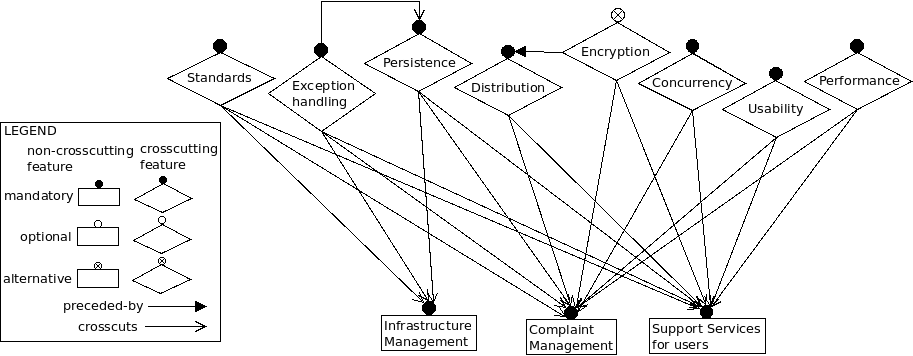
\includegraphics[scale=0.4]{figs/aofv.png}
   \caption{Aspect-oriented feature view}
   \label{fig:aofv}
\end{figure}

\section{Design}
\label{sec:design}
%TODO por que nao usei o Zhang et al. ICCSSE 2008
Figure~\ref{fig:design} shows activities necessary to build the PLA based on analysis documents. In order to create the PLA, the feature
diagram endures four transformations, which are based on the Feature-Architecture Mapping (FArM) method~\cite{Sochos:2006:FAM}. FArM
considers only the feature diagram to create the PLA. We extended FArM in order to consider the crosscutting concerns which are represented
in the AOFV. Thus, transformations applied to the feature diagram are also applied to the AOFV.  


\begin{figure}[!htb]
   \centering
   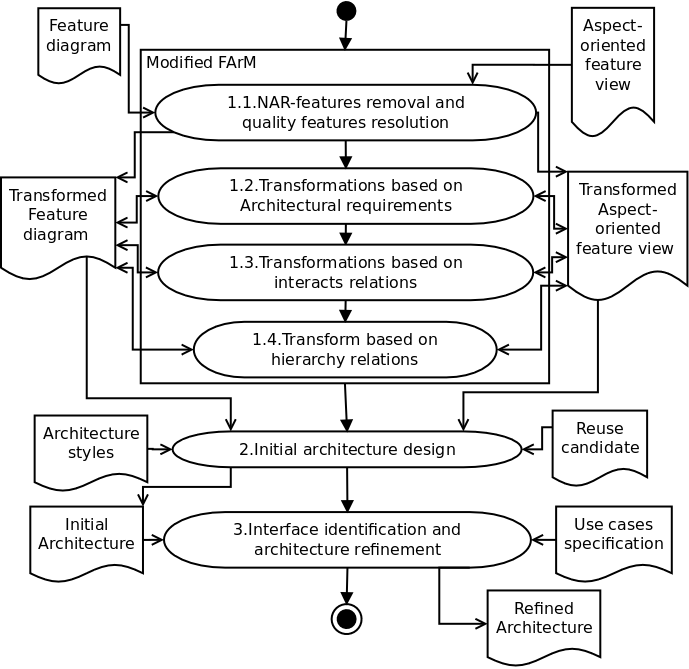
\includegraphics[scale=0.3]{figs/design-v01.png}
   \caption{Design activities}
   \label{fig:design}
\end{figure}



\subsection{From feature model to architecture model}
\label{sec:farm}

Deriving the PLA from use cases induces feature scattering and tangling~\cite{Sochos:2006:FAM}. The Feature-Architecture Mapping (FArM)
method~\cite{Sochos:2006:FAM} supports the design of PLA based on feature diagram. FArM defines 4 transformations to build the architecture
based on feature diagram: 

\begin{enumerate}
\item \textbf{Tranformation 1.} Removing non-architecture related features  and Resolving quality features (Section~\ref{sec:removingNAR})
\item \textbf{Tranformation 2.} Transforming based on architectural requirements (Section~\ref{sec:transfArchReq})
\item \textbf{Tranformation 3.} Transforming based on interacts relations (Section~\ref{sec:transInteracts})
\item \textbf{Tranformation 4.} Transform based on hierarchy relations (Section~\ref{sec:transfHierRel})
\end{enumerate}

 
\subsubsection{Removing non-architecture related features and Resolving quality features}
\label{sec:removingNAR}

According to van der Linden et al.~\cite[Chapter 3.1.2]{Linden:2007:SPL}, one important issue related to architectures is architectural
significant requirements, which encompass two types of requirements: functional requirements and quality requirements. Functional
requirements determine \textit{what} is realised and quality requirements determine \textit{how} it is realised~\cite[Chapter
3.1.2]{Linden:2007:SPL}. Non-architecture related (NAR) features are the opposite of architectural significant requirements.

In the Public Health Complaint SPL, all subfeatures of \textit{Computer infrastructure} (except \textit{Java RMI}, \textit{Java Servlets},
and \textit{Database}) and subfeatures of \textit{Compatibility} are NAR features. 

FArM method resolves quality features (i.e. a feature that represents a quality attribute) through the integration with existing
functional features. In the Public Health Complaint SPL, the following quality features are integrated with existing
functional features: \textit{Persistence}, \textit{Usability}, \textit{Distribution}, \textit{Concurrency}, \textit{Availability},
\textit{Encryption}, and
\textit{Performance}. \textit{Persistence} is composed by \textit{Database}, which can be implemented by either \textit{MySQL} or
\textit{Oracle}. \textit{Usability} is composed by \textit{User interface}, which is implemented by \textit{Java Servlets}. For instance,
\textit{Distribution} can be implemented by both \textit{Java RMI} and \textit{Java Servlets} features. \textit{Java RMI} can also implement
\textit{Encryption} feature, a subfeature of \textit{Security}. \textit{Concurrency} is implemented by \textit{Java Synchronization}
mechanisms~\cite{java}. \textit{Availability} is supported by the implementation of \textit{Exception Handling}.

\textit{Performance} feature and its subfeature depends on architecture styles~\cite[Chapter
4.1]{Bass:1998:SAP}. However, we believe that, for Public Health Complaint SPL, the performance requirement (see NFR03) should not be a
driving requirement for defining the product line architecture (PLA). Healthwatcher legacy architecture (Section~\ref{sec:designRecovery})
is a layered architecture, which is not performance-friendly architecture style. Furthermore, Healthwatcher implementation~\cite{hw-tao}
does not support any mechanism to improve performance, like the implementation of cache. Figure~\ref{fig:step1} in
Appendix~\ref{sec:app-farm} shows the result of transformation 1, which includes removing NAR features (Section~\ref{sec:removingNAR}) and
resolving quality attributes.

\subsubsection{Transforming based on architectural requirements}
\label{sec:transfArchReq}

There may exist architectural requirements that must be satisfied through direct resolution, that is, integrating with existing functional
features. As architectural requirements have already been specified as features, no feature has been added.

\subsubsection{Transforming based on interacts relations}
\label{sec:transInteracts}
After transformations described in steps 1 to 3, current feature model contains exclusively functional features. The communication among
these features is represented by introducing new features relation, namely the interacts relation~\cite{Sochos:2006:FAM}. FArM
defines the following interacts relation:

\begin{itemize}
\item \textbf{Type 1.} It connects two features where one features uses the other feature's functionality.
\item \textbf{Type 2.} It connects two features where the correct operation of one feature alters the behavior of the other feature.
\item \textbf{Type 3.} It connects two features where the correct operation of one feature contradicts with the correct operation of the
other feature.
\end{itemize}

Before adding interacts relations among features, it is important to check if the relation already exists in the AOFV. If any type of
interacts relation has a correspondent in AOFV, it must not be added to the feature model. For instance, \textit{Complaint Management} and
its subfeatures uses \textit{Database} feature in order to persist data. According to FArM, an \textit{uses} relation would be added between
\textit{Complaint Management} and \textit{Database}. However, in AOFV it is already represented that \textit{Database} (which is the
implementation of \textit{Persistence} crosscutting feature) crosscuts \textit{Complaint Management}. Although the semantic of uses and
crosscuts relations are different Thus, it is not necessary to add the \textit{uses} relation because it is already represented
in the AOFV. 

Note that \textit{crosscuts} relations (type 4) modifies features, which is similar to \textit{alters} relation (type 2) defined in FArM
method~\cite{Sochos:2006:FAM}. Whereas the \textit{crosscuts} is a relation between one
crosscutting feature and other features (1-n relation), \textit{alters} is a relation between two features (1-1 relation).

After the identification of relations between features, they are transformed based on two criteria:
\begin{itemize}
\item Criterion 1. The type of interacts relations.
\item Criterion 2. The number of interacts relations.
\end{itemize}


\subsubsection{Transform based on hierarchy relations}
\label{sec:transfHierRel}
In this step, features are grouped to become components. 
The module hierarchy largely corresponds to the feature hierarchy~\cite{Kang:1998:FFR}

\begin{enumerate}
\item If a feature does not have any sibling and it is not the root feature, merge the feature with its parent recursively;
\item All parent-features should become components (except the root feature) and their subfeatures should become either subcomponents or
classes depending on how complex it is to implement them. Note that this step can be recursively applied.
\item All the relationships between subfeatures must be represented as relationships between components. If a subfeature has become a
subcomponent  their respective superfeatures of the same level\footnote{The
level of a feature is given by the shortest distance between the feature and the root feature.}.
\end{enumerate}



% depois que foi definida uma arquitetura de referencia e que os componentes foram identificados, eles devem ser colocados adequadamente de
% acordo com os atributos de qualidade da arquitetura

\begin{figure}[h!t!b!]
   \centering
    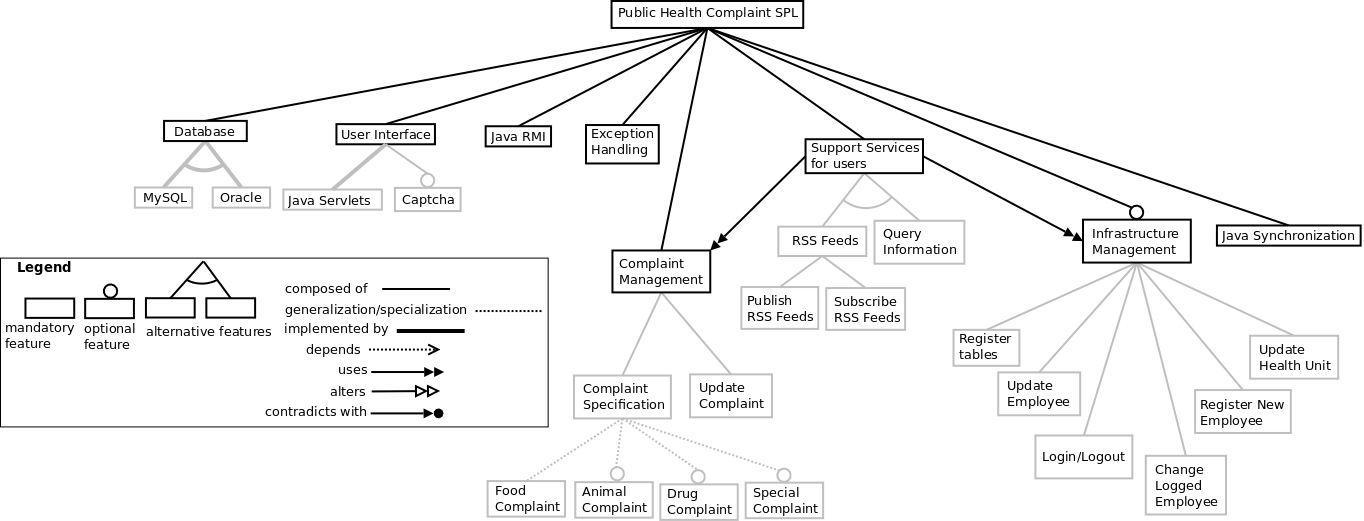
\includegraphics[scale=0.23]{figs/phs-farm-step4-v04.png}
   \caption{Transformation 4: Grouped features and their relationships}
   \label{fig:groupedFeat}
\end{figure}


\subsubsection{Aspect-oriented feature transformations}
\label{sec:farm-aofv}

The AOFV extends the feature model in order to support reasoning about crosscutting features. Thus, the transformations describe in
Section~\ref{sec:farm} must also be applied to the AOFV. For instance, the first transformation of FArM (Section~\ref{sec:removingNAR}), NAR features
are removed from the feature model causing the same effect on AOFV. 

% \item \textbf{Type 4.} It connects two features where one crosscuts the other.
% \item \textbf{Type 5.} It connects two features where one is preceded by the other regarding their influence on a third feature.


\begin{figure}[h!t!b!]
   \centering
    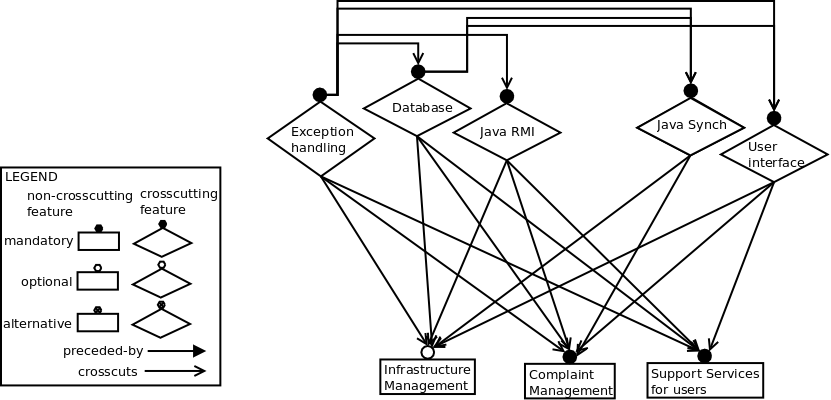
\includegraphics[scale=0.3]{figs/aofv-step4-v03.png}
   \caption{Aspect-oriented feature view after FArM transformations}
   \label{fig:aofv-farm-step4}
\end{figure}

\subsection{Initial architecture design}

After transforming the feature diagram according to FArM (Section~\ref{sec:farm}) and propagating these transformations to the AOFV
(Section~\ref{sec:farm-aofv}), we merged both diagrams in order to define all relations among features.

\begin{figure}[h!t!b!]
   \centering
    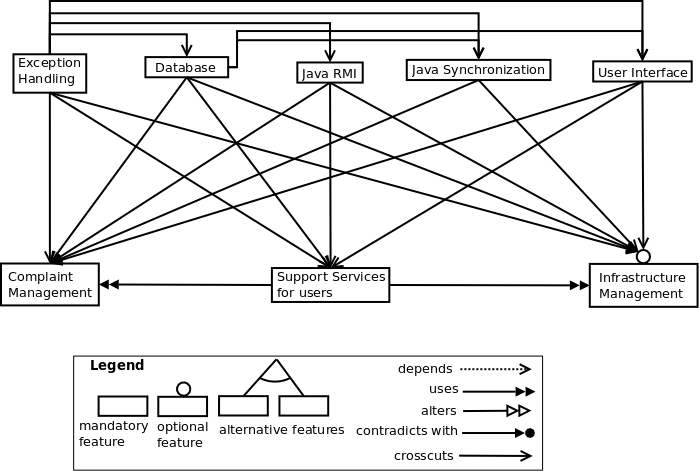
\includegraphics[scale=0.35]{figs/merge-fm-aofv-v01.png}
   \caption{Concept model}
   \label{fig:conceptModel}
\end{figure}



\subsection{Interface identification and architecture refinement}
\label{sec:archRefinement}
Since we intend to Public Health Complaint SPL based on components, it is known that components communicate through their interfaces.
In this context, interfaces are usually classified in provided and required interfaces~\cite{Szyperski:2002:CS}. However, aspects provide
another mechanism to establish the communication among components, because an aspect can capture a method call to an interface, for
instance. Some works in the literature propose a new aspect-oriented interface, which Griswold et al. called
crosscutting programing interface (XPI)~\cite{Griswold:2006:MSD}, which allows the communication among components. Thus, there are two types
of interfaces: regular interfaces which are designed and implemented by object-oriented techniques and XPIs which
are designed and implemented by aspect-oriented techniques.

The \textit{crosscuts} relations have at one end an XPI which exposes the joinpoints of the component and at other end an Abstract aspect
which has the advices. Abstract aspects are connected to XPIs through aspect-connectors.


\begin{itemize}
 \item \textit{crosscuts} relations between components must be mediated by using aspect-orientation, that is, the crosscut component must
have an XPI and the component which cuts across other components must have an Abstract aspect.
\item \textit{uses}, \textit{alters}, and \textit{contradicts with} relations must be mediated by using object-orientation, that is,
regular provided and required interfaces.
\end{itemize}


\begin{figure}[h!t!b!]
   \centering
    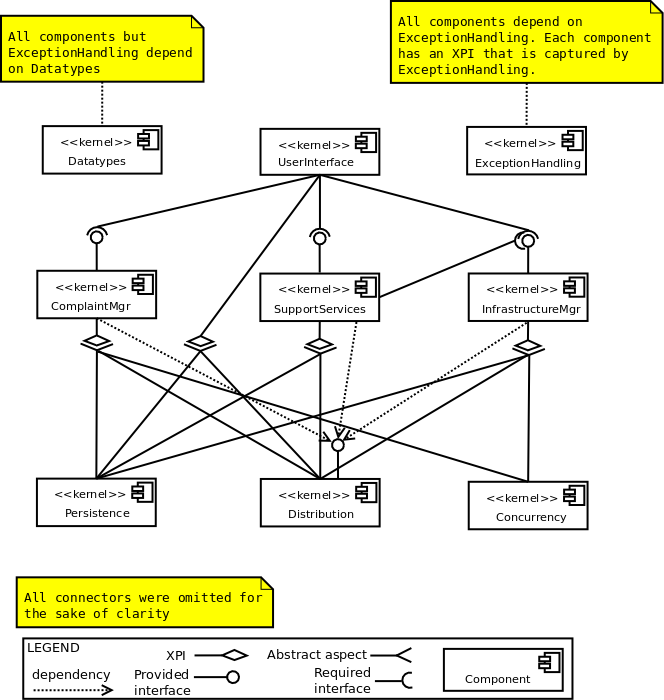
\includegraphics[scale=0.35]{figs/phc-pla-v01.png}
   \caption{Initial product line architecture specification}
   \label{fig:initialArch}
\end{figure}

Architecture refinement is performed by refining the identified interfaces using UML communication diagrams. Eler and Masiero proposed an approach to
refine component interfaces
using communication diagrams~\cite{Eler:2006:AC}. We extended their approach to use XPIs to realize use case extensions (see
Section~\ref{sec:analysis}). The use of XPIs and
abstract aspects minimizes the coupling between components~\cite{Dias:2010:LAC}. One input for this activity is the \textit{Use case specification},
which allows to reason about
the behavior of the architectural components and it specifies what information each interface needs. 


% quando dois componentes entrecortarem um mesmo terceiro componente e houver uma relacao de precedencia entre os componentes, a conexao
% entre os tres deve ser feita por meio de um unico conector, onde o conflito sera resolvido estabelecendo a precedencia adequadamente.

\section{Provisioning}

As shown in Figure~\ref{fig:provisioning}, in this approach \textit{Provisioning} consists of the following activities: \textit{Evaluation of legacy
components}, \textit{Component
implementation and refactoring}, and \textit{Connector specification and implementation}. The objective of evaluating legacy components is to increase
reuse and reduce costs and time-to-market. The
quality of legacy components must be evaluated. Metrics such as coupling, cohesion, complexity, and dependency can be collected by
tools~\cite{Lee:2009:ERU} and are useful to
evaluate the quality of a component.

\begin{figure}[!htb]
   \centering
   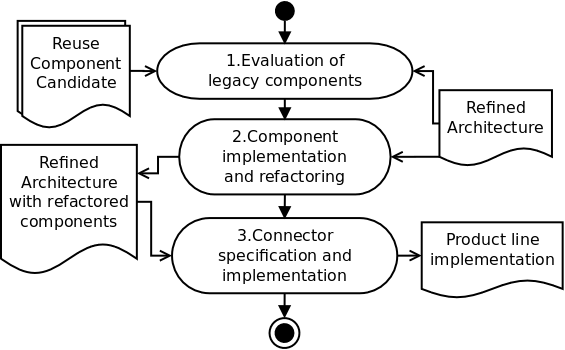
\includegraphics[scale=0.3]{figs/provisioning.png}
   \caption{Provisioning activities}
   \label{fig:provisioning}
\end{figure}

\subsection{Evaluation of legacy components}
The objective of evaluating legacy components is to increase reuse and reduce costs and time-to-market. The quality of legacy components must be
evaluated. Metrics such as coupling, cohesion, complexity, and dependency can be collected by tools~\cite{Lee:2009:ERU} and are useful to
evaluate the quality of a component.

\subsection{Component implementation and refactoring}
The \textit{Component Implementation and Refactoring} activity is responsible for implementing new features and refactoring components that
implement reused features. Some components might be reused without any
modifications. Others might be wrapped using a different component model in order to make them compliant to the current PLA.

We managed to reuse components that implement the Healthwatcher features, but we also had to implement features that do not belong to
Healthwatcher, such as \textit{RSS Feeds} and \textit{Captcha}. Reused components were refactored to adapt to current PLA. Refactoring is a technique
for changing the internal structure of existing programs to make them easier to understand and cheaper to
modify, wihtout changing their observable behavior~\cite{Fowler:1999:RID}. During refactoring, we avoided changing legacy code. Instead, we wrapped
legacy code using COSMOS*-VP component model~\cite{Dias:2010:LAC}.


\subsection{Connectors specification and implementation}
Finally, \textit{Connectors specification and implementation} activity has a main role for variability specification and implementation, because
connectors are used to materialize
variability. Moving the implementation of variability decisions from components to connectors supports PLA evolution~\cite{Tizzei:2011:ECSA}. The
COSMOS*-VP component implementation model~\cite{Dias:2010:LAC} provides guidelines to implement components that handle both regular and
aspectual communication and it also supports the design and implementation of such connectors to encapsulate variability decisions. 

\section{Data collection and analysis}

Metrics have been collected  based on legacy Healthwatcher (Legacy-HW) application and Healthwatcher product which was derived from Public Health
Complaint SPL (PHC-HW). 

We have collected 9 metrics, which can be divided in two groups: (i)~size metrics, namely, number of modules, number of components, number of
connectors, number of features, total number of Lines of Code (LOC), average LOC/module; and (ii) evolution metrics, namely, feature tangling, feature
scattering, and average efferent coupling between modules (coupling for short). A module can be either a component or a connector. 

Metrics of number of modules, number of components, and number of connectors have been manually collected based on architectures. Legacy-HW is
presented in Section~\ref{sec:designRecovery} while PHC-HW is an instantiation of Public Health Complaint PLA presented in
Section~\ref{sec:archRefinement}. The number of features was collected by counting them in Table~\ref{tab:featOfEachProd}. We collected the total
number of LOC using shell scripts (see Appendix~\ref{sec:app-scripts}). Blank lines and comments were also counted.

Separation of concerns is one measurable attribute of evolution~\cite{Brcina:2009:OPM}. In order to measure separation of concerns, we have used
metrics presented by Riebisch and
Brcina~\cite{Riebisch:2008:ODV}. Equation~\ref{eq:sca} shows how to measure the number of modules ($a \in A$) that implements a particular
feature $f \in F$. Note that the equation considers the ideal case where no scattering of features exists by the subtraction of 1.

\begin{equation}\label{eq:sca}
sca(f):=|{a:f\rightsquigarrow a}|-1 
\end{equation}

Equation shows how it is measured the scattering of one feature, while Equation~\ref{eq:fsca} shows how it is measured the
scattering of all features. The scattering of variation points and tangling of features are measured similarly. The higher is
the
scattering, the worse is the support
for PLA evolution.

\begin{equation}\label{eq:fsca}
fsca(F):= \frac{\sum_{f\in F}sca\{f\}}{|F|\cdot|A|}, fsca \in [0,1)
\end{equation}

The complete matrix that shows the mapping between features and modules is available on Public Health Complaint website~\cite{phc}.

Efferent coupling refers to the degree of interdependence between parts of a design~\cite{Chidamber:1994:MSO}, which means that a high
interdependence can harm maintainability. In this study, we have measured the efferent coupling between modules, that is, the number of modules each module knows.
The collection of coupling metrics was supported by shell scripts (see Appendix~\ref{sec:app-scripts}).

\section{Related work}

\subsection{Features and aspects}
Kastner

Lee et al. propose a way to combine feature-oriented analysis (FOA) and aspect-oriented programming (AOP). AOP can be used to implement crosscutting
features (i.e. optional and alternative features) . AOP addresses the dependency between features by encapsulating dependencies related to a variable
feature into the aspect implementing the variable feature

\subsection{Extractives approaches}

Lee ICSR'10

Niu RE'08



\subsection{Empirical studies}

\section*{Acknowlegedments}
Leonardo P. Tizzei is supported by CAPES - Brazil. Cec\'{i}lia M.F. Rubira is partially supported by Fapesp - Brazil and CNPQ - Brazil. We
also thank the Healthwatcher developers: Phil Greenwood, Thiago Bartolomei, Eduardo Magno, Uir\'{a} Kulesza, S\'{e}rgio Soares, Nelio
Cacho, and Marcos D\'{o}sea.



\appendix

\section{From feature diagram and aspect-oriented feature view to product line architecture}
\label{sec:app-farm}

\begin{figure}[h!t!b!]
   \centering
   \rotatebox{90}{    
   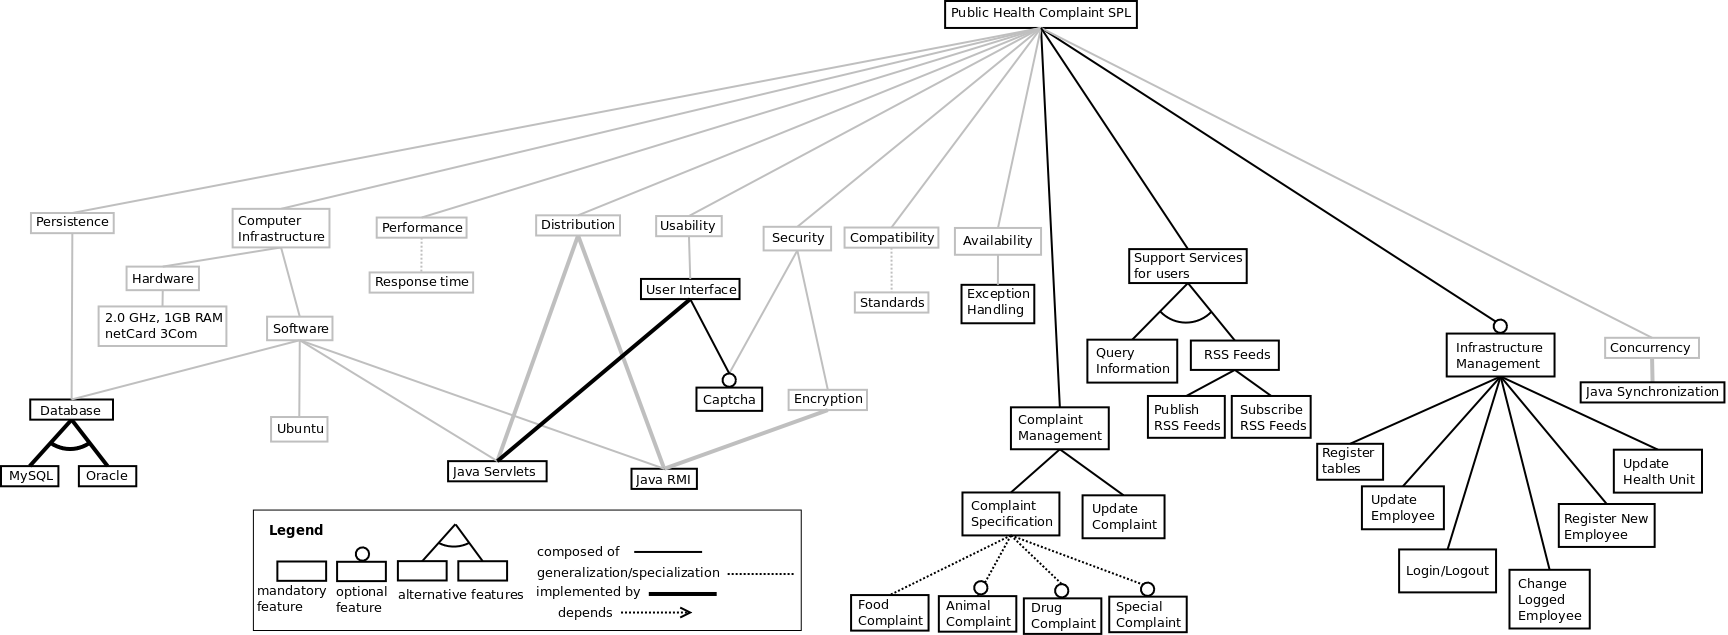
\includegraphics[scale=0.27]{figs/phs-farm-step1-v03.png}
   }
   \caption{FArM transformation 1}
   \label{fig:step1}
\end{figure}

\begin{figure}[h!t!b!]
   \centering
   \rotatebox{90}{    
   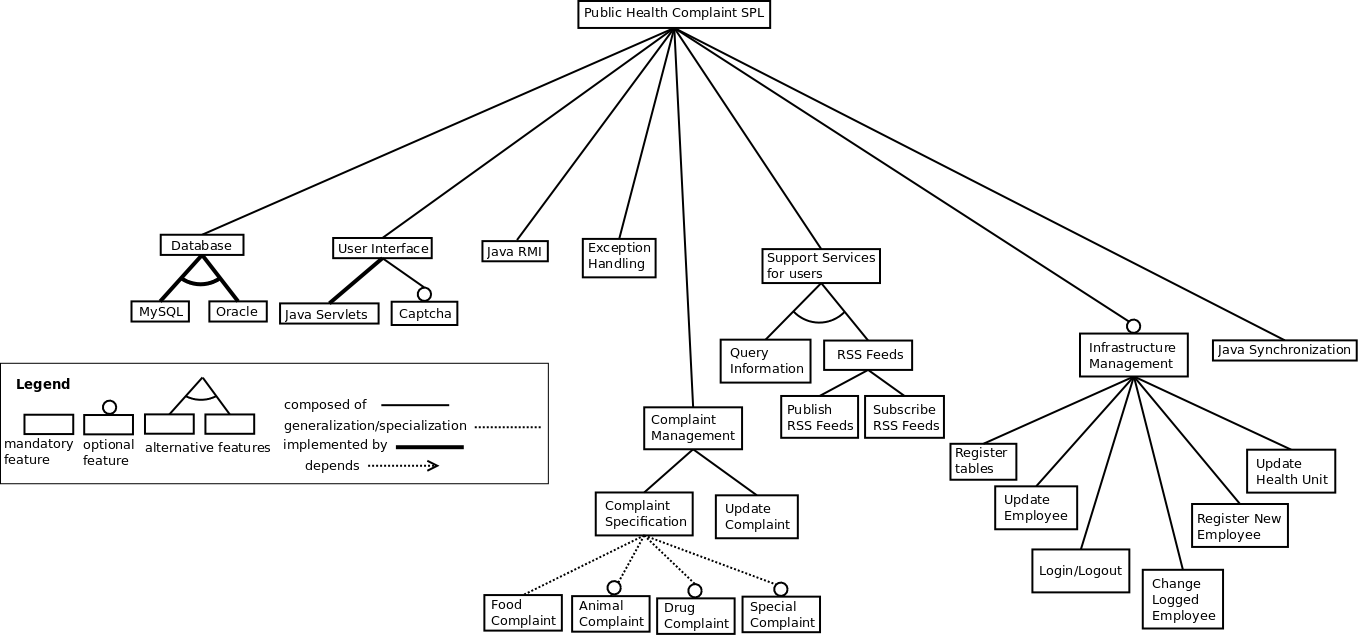
\includegraphics[scale=0.27]{figs/phs-farm-step2-v04.png}
   }
   \caption{FArM transformation 2}
   \label{fig:step2}
\end{figure}

\begin{figure}[h!t!b!]
   \centering
   \rotatebox{90}{    
   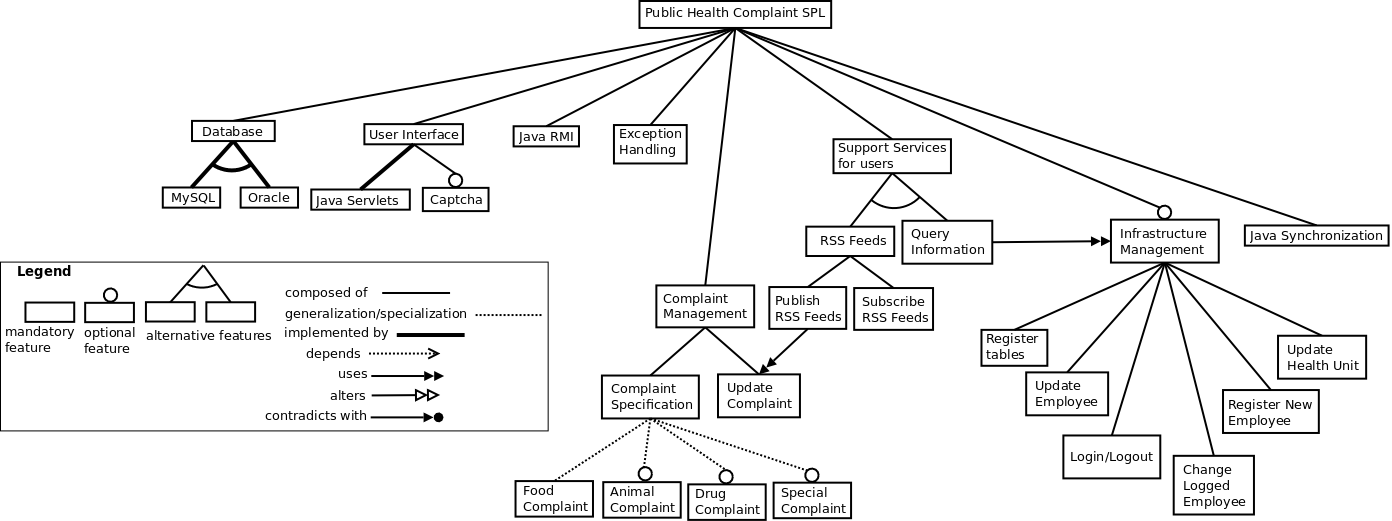
\includegraphics[scale=0.3]{figs/phs-farm-step3-v04.png}
   }
   \caption{FArM transformation 3}
   \label{fig:step3}
\end{figure}

\begin{figure}[h!t!b!]
   \centering
   \rotatebox{90}{    
   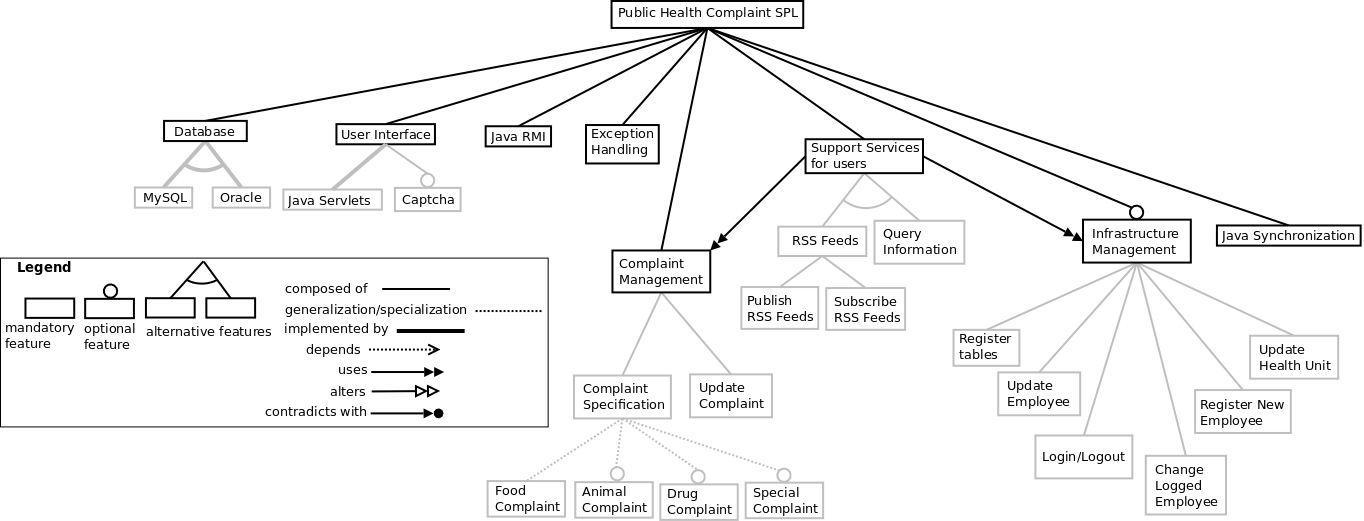
\includegraphics[scale=0.3]{figs/phs-farm-step4-v04.png}
   }
   \caption{FArM transformation 4}
   \label{fig:step4}
\end{figure}


\section{Scripts}
\label{sec:app-scripts}
\lstset{ %
language=bash,                % the language of the code
basicstyle=\footnotesize,       % the size of the fonts that are used for the code
numbers=left,                   % where to put the line-numbers
numberstyle=\footnotesize,      % the size of the fonts that are used for the line-numbers
stepnumber=2,                   % the step between two line-numbers. If it's 1, each line 
}

To count the number of LOC, the script described in Figure~\ref{lst:countCode} was executed. It counts the number of LOC, including blank lines and
comments, of all files whose extensions are either \texttt{.java} (Java files) or \texttt{.aj} (AspectJ files). However, the result has a minor error,
because the
execution of this script adds 3 lines to each file it reads. Thus, the second script, described in Figure~\ref{lst:countFile}, counts the number of
files read in order to collect the correct value. 

\begin{figure}

\begin{lstlisting}
find <application source folder> -name "*.java" -or -name "*.aj" | xargs more | wc
\end{lstlisting}
\caption{The above  script counts the LOC of all files whose extensions are either .java or .aj}
\label{lst:countCode}
\end{figure}

\begin{figure}
\begin{lstlisting}
find <application source folder> -name "*.java" -or -name "*.aj" | wc
\end{lstlisting}
\caption{The above  script counts the number of files whose extensions are either .java or .aj}
\label{lst:countFile}
\end{figure}

Figure~\ref{lst:coupling} shows the script we created to support the collection of coupling metric. The script below was executed to collect data from PHC-HW,
but the script to collect data from Legacy-HW was slightly different. The script reads all \texttt{.java} and \texttt{.aj} files and selects only references to other packages. As in COSMOS*-VP each module has a corresponding package, then it is possible to know the relations between modules analyzing the \texttt{import} of all classes and aspects of each module.
The result is stored in a file, one for each module. This file is analyzed to find out the coupling between modules.

\begin{figure}
\begin{lstlisting}
#!/bin/bash/
   for i in $( ls ); do
      find $i -name "*.java" -or -name "*.aj" | xargs more | grep -E publichealthcomplaint. 
      | grep -v publichealthcomplaint.$i | sort -nk 2 > $i.txt
   done
\end{lstlisting}
\caption{The above script supports the collection of coupling metric}
\label{lst:coupling}
\end{figure}




\bibliography{refPublicHealth}
\bibliographystyle{plain}

\end{document}
